\documentclass[journal]{IEEEtran}

% ================ IEEE REQUIRED PACKAGES =================
\usepackage{cite}
\usepackage{amsmath,amssymb,amsfonts}
\usepackage{graphicx}
\usepackage{textcomp}
\usepackage{xcolor}
\usepackage{booktabs}
\usepackage{array}
\usepackage{tabularx}
\usepackage{multirow}
\usepackage{makecell}
\usepackage{subcaption}
\usepackage{url}
\usepackage[hidelinks]{hyperref}

% Multi-directory image search path to ensure all figures resolve cleanly
\graphicspath{{figures/}{paper/figures/}{Research paper/}{./}}

% Table column helpers
\newcolumntype{Y}{>{\raggedright\arraybackslash}X}
\newcolumntype{P}[1]{>{\raggedright\arraybackslash}p{#1}}

% Image helper macro: loads figure or renders a clear placeholder if file is missing
\newcommand{\insertfigure}[2]{%
  \IfFileExists{#1}{%
    \includegraphics[width=\linewidth,height=0.75\textheight,keepaspectratio]{#1}%
  }{%
    \fbox{\parbox[c][3.0cm][c]{0.92\linewidth}{%
    \centering\textbf{FIGURE: \texttt{\detokenize{#1}}}\\[4pt]
    \small #2}}%
  }%
}

\begin{document}

\title{AI-Based Cloud Network Intrusion Detection System Using Lightweight Hybrid Autoencoder and XGBoost with Real-Time Drift Adaptation}

\author{Ansh~Pawaskar,
        Nesar~Naik,
        and~Tejaswini%
\thanks{The authors are with the Department of Artificial Intelligence and Machine Learning, Manipal Institute of Technology, Manipal Academy of Higher Education, Manipal 576104, Karnataka, India (e-mail: anshpawaskar21@gmail.com, naiknesar521@gmail.com).}%
\thanks{Manuscript received \today; revised \today.}%
}

\markboth{IEEE Transactions on Information Forensics and Security,~Vol.~XX, No.~X, \today}%
{Pawaskar \MakeLowercase{\textit{et al.}}: AI-Based Cloud Network Intrusion Detection System}

\maketitle

% =================================================
\begin{abstract}
Network intrusion detection systems (NIDSs) face an enduring operational trade-off: supervised classifiers deliver near-perfect discrimination on closed-world benchmarks but fail against unseen zero-day attacks, whereas unsupervised anomaly detectors capture novel deviations at the expense of elevated false-alarm rates and uncalibrated decision thresholds. Furthermore, data leakage and arbitrary Gaussian thresholding ($\mu + 3\sigma$) frequently inflate published laboratory accuracy while concealing operational blindspots. This paper presents a leakage-free hybrid NIDS combining an unsupervised deep symmetric Autoencoder ($128\text{--}64\text{--}32\text{--}16$) trained exclusively on benign traffic with an extreme gradient boosted decision tree (XGBoost) classifier and alert-gated TreeSHAP explainability. Evaluated on strictly deduplicated partitions of CICIDS2018 ($671{,}131$ unique flows) and NSL-KDD ($147{,}790$ instances) enforcing an absolute zero-leakage invariant ($\text{Train} \cap \text{Test} = \emptyset$), the framework uses validation-guided Youden's $J$ thresholding to eliminate the zero-recall collapse of rigid sigma rules, securing 99.70\% attack recall. Under a Leave-One-Attack-Out (LOAO) protocol, the anomaly gatekeeper successfully flags 93.11\% of unseen DoS and 82.22\% of unseen Probe attacks without prior supervised exposure. Profiling on native multi-core CPU architecture confirms an end-to-end inference latency of 0.1830~ms per flow ($5{,}464$~flows/s throughput) and a peak memory footprint of 527.0~MB Resident Set Size (RSS), demonstrating the practical feasibility of explainable defense-in-depth on commodity enterprise hardware.
\end{abstract}

\begin{IEEEkeywords}
Network intrusion detection, CICIDS2018, NSL-KDD, autoencoder, XGBoost, anomaly screening, TreeSHAP, operational latency, zero-day generalization.
\end{IEEEkeywords}

% =================================================
\section{Introduction}
\IEEEPARstart{M}{odern} enterprise networks and multi-tenant cloud ecosystems contend with an unprecedented velocity of volumetric, multi-vector cyber intrusions \cite{raza2024,abdallah2024,rm2023}. Traditional signature-based defenses provide robust protection against historical exploits but remain fundamentally blind to zero-day mutations and stealthy scanning activities \cite{ahmed2025,markevych2023,sowmya2023}. Consequently, security operations centers (SOCs) have increasingly shifted toward machine learning (ML) and deep learning (DL) paradigms capable of learning complex traffic representations from high-dimensional network flow records \cite{diana2025,hozouri2025,ahmed2026}. Recent surveys underscore the promise of hybrid systems that combine unsupervised representation learning with supervised classification across diverse edge, IoT, and cloud perimeters \cite{kamal2026,alsubaei2025,mallidi2025,vinayaka2025}.

\subsection{Problem Statement and Research Gap}
Despite encouraging published benchmark results, standard ML-based NIDS implementations exhibit critical systemic vulnerabilities. First, purely supervised tree ensembles (such as XGBoost or Random Forests) operate under the strict \textit{closed-world assumption}; while they achieve near-perfect classification on known signatures, their detection accuracy collapses entirely when presented with unseen attack classes \cite{abdulganiyu2024,sajid2024}. Second, unsupervised Autoencoders intended for anomaly detection predominantly rely on rigid Gaussian thresholding rules ($\mu + 3\sigma$) or arbitrary percentiles. On heavy-tailed, non-Gaussian network error distributions, these static rules cause catastrophic threshold inflation, reducing attack recall to near-zero. Third, prevalent benchmark practices suffer from subtle cross-partition data leakage (identical flow duplicates shared between training and test sets), masking real-world operational degradation \cite{arcos2025,hussein2026}. Finally, state-of-the-art Explainable AI (XAI) frameworks incur prohibitive computational overhead when applied naively to every line-rate packet, causing throughput collapse in real-time monitors \cite{neupane2022,benncir2024,mahmoud2025}.

\subsection{Research Objectives and Scope}
To resolve this dichotomy, this study designs, validates, and profiles a two-stage hybrid NIDS that pairs benign-trained Autoencoder reconstruction gating with multi-class XGBoost classification and selective, alert-triggered TreeSHAP explainability. The specific research objectives are:
\begin{enumerate}
\item Establish an audited, cryptographically verified zero-leakage preprocessing pipeline ($\text{Train} \cap \text{Test} = \emptyset$) on CICIDS2018 and NSL-KDD.
\item Develop a deep symmetric Autoencoder trained exclusively on benign network flows to serve as a line-rate anomaly gatekeeper.
\item Overcome parametric threshold collapse via validation-guided Youden's $J$-index optimization paired with an isolated benign sliding-window buffer.
\item Quantify open-world defense-in-depth through an empirical Leave-One-Attack-Out (LOAO) protocol and chronological temporal partitioning.
\item Profile end-to-end CPU execution latency, throughput, and Resident Set Size (RSS) memory consumption to ensure operational deployment viability.
\end{enumerate}

% =================================================
\section{Related Work}

\subsection{Machine Learning and Autoencoders in NIDS}
Extensive research has investigated supervised and unsupervised learning for intrusion detection \cite{diana2025,ahmed2026,sowmya2023}. Unsupervised Autoencoders compress network flow vectors into low-dimensional latent bottlenecks, using the reconstruction error $e(\mathbf{x}) = \frac{1}{d}\|\mathbf{x}-\hat{\mathbf{x}}\|^2$ to quantify deviations from normal operational behavior \cite{abdallah2024,shree2025}. While effective at identifying unmodeled statistical anomalies, standalone Autoencoders cannot discriminate among specific threat categories (e.g., distinguishing brute-force attempts from volumetric denial-of-service) and frequently suffer from elevated false-positive rates (FPR) when normal traffic exhibits natural variance \cite{hussein2026,kamal2026}.

\subsection{Hybrid Architectures and Supervised Classifiers}
To provide actionable threat intelligence, hybrid frameworks integrate deep representations with supervised tree ensembles \cite{sajid2024,shirley2025,vinayaka2025}. Abdulganiyu et al. \cite{abdulganiyu2024} utilized Variational Autoencoders for data oversampling in conjunction with XGBoost, while Hussein and R\'ep\'as \cite{hussein2026} paired Autoencoders with Gaussian Mixture Models. However, existing hybrid pipelines often evaluate models under artificial i.i.d. assumptions without verifying whether the anomaly gate preserves attack traffic or whether live socket captures match offline feature extractors \cite{arcos2025,amin2025}.

\subsection{Explainability and Computational Feasibility}
Interpreting high-stakes security alerts is essential for security analysts \cite{neupane2022,ghosh2026}. Post-hoc attribution frameworks, such as SHAP and LIME, provide local additive feature importance \cite{benncir2024,mahmoud2025}. Nevertheless, computing SHAP values over multi-thousand flow streams introduces severe latency penalties. Gating attribution exclusively to confirmed anomalous events represents a necessary architectural pivot toward line-rate explainability \cite{mahmoud2025,vinayaka2025}.

% =================================================
\section{Research Gap and Literature Comparison}
Table~\ref{tab:gap} synthesizes ten foundational reference investigations against the specific contributions and experimental scope of this study.

\begin{table*}[!t]
\centering
\caption{Comparison of Relevant Foundational Studies and Research Gaps Addressed by This Study.}
\label{tab:gap}
\scriptsize
\setlength{\tabcolsep}{3pt}
\renewcommand{\arraystretch}{1.2}
\begin{tabularx}{\textwidth}{P{0.14\textwidth}P{0.13\textwidth}P{0.12\textwidth}P{0.11\textwidth}P{0.12\textwidth}P{0.13\textwidth}Y}
\toprule
\textbf{Paper} & \textbf{Problem} & \textbf{Method} & \textbf{Dataset} & \textbf{Reported Result} & \textbf{Limitation} & \textbf{Gap Addressed by This Study}\\
\midrule
Abdallah et al. (2024) \cite{abdallah2024} & Cloud network anomaly detection & Review of ML/DL paradigms & Multi-benchmark survey & Qualitative taxonomy & Broad survey without direct empirical pipeline benchmark & Controlled evaluation of a unified two-stage pipeline on CPU.\\
Abdulganiyu et al. (2024) \cite{abdulganiyu2024} & Imbalanced intrusion traffic & VAE data synthesis + XGBoost & NSL-KDD, CICIDS2018 & Binary Acc = 99.8\% & VAE utilized strictly for synthesis, not anomaly gating & Tests the empirical defensive value of benign reconstruction gating.\\
Neupane et al. (2022) \cite{neupane2022} & Explainability of NIDS alerts & Survey of X-IDS methods & Benchmark survey & XAI framework & No operational latency or stability quantification & Quantifies alert-gated TreeSHAP latency and Jaccard stability.\\
Ben Ncir et al. (2024) \cite{benncir2024} & Interpretable deep detection & Ensemble 1D-CNN/LSTM + SHAP & NSL-KDD & Acc = 97.05\%, F1 = 97.19\% & Heavy recurrent unrolling; unverified attribution stability & Sub-millisecond tree-gated XAI with verified attribution stability.\\
Mahmoud et al. (2025) \cite{mahmoud2025} & Explainable two-stage IDS & XI2S-IDS Staged Model & UNSW-NB15, CICIDS2017 & Acc = 97.0\%, F1 = 97.2\% & Global per-flow SHAP creates throughput bottleneck & Restricts XAI strictly to anomaly alerts ($RE > \tau^*$).\\
Sajid et al. (2024) \cite{sajid2024} & Scalable hybrid detection & Hybrid Deep Learning + ML & Benchmark pools & Acc = 97.91\%, F1 = 87.09\% & Lacks temporal non-stationarity and drift evaluation & Evaluates chronological temporal shifts and LOAO unseen attacks.\\
Shirley and Priya (2025) \cite{shirley2025} & Evolving IoT threats & Autoencoder--FNN fusion & CICIoT2023 & Acc = 99.55\%, F1 = 90.91\% & Static thresholding heuristic vulnerable to shift & Analyzes Pareto-optimal threshold calibration via Youden's $J$.\\
Hussein and R\'ep\'as (2026) \cite{hussein2026} & Multi-class threat classification & Deep AE + GMM + XGBoost & NSL-KDD, UNSW-NB15 & F1 > 0.94, AUC > 0.97 & GMM clustering introduces significant inference delay & Replaces heavy density estimators with direct reconstruction gating.\\
Diana et al. (2025) \cite{diana2025} & Network IDS evolution & Comprehensive architectural survey & Literature survey & Survey conclusions & Broad coverage without standardized leakage audit & Enforces cryptographically verified zero cross-split leakage.\\
Arcos-Argudo et al. (2025) \cite{arcos2025} & Classical vs hybrid representations & Comparative AE + Linear Models & NSL-KDD, CICIDS2017 & AUC = 0.9043, F1 = 0.7583 & Restricted to linear downstream classifiers & Pairs non-linear Autoencoder with gradient-boosted trees.\\
\bottomrule
\end{tabularx}
\end{table*}

% =================================================
\section{Proposed Methodology}

\subsection{System Architecture}
The framework operates as a pipelined detection system: incoming network traffic is parsed into bidirectional flow records, preprocessed through training-locked transformers, screened by an unsupervised Autoencoder, selectively classified by XGBoost upon anomaly detection, and explained via alert-gated TreeSHAP (Fig.~\ref{fig:architecture}).

\begin{figure*}[!t]
    \centering
    \insertfigure{simple_architecture.png}{Proposed Autoencoder--XGBoost Architecture}
    \caption{Proposed Autoencoder--XGBoost architecture illustrating leakage-free data ingestion, reconstruction gating, adaptive sliding buffer, multi-class XGBoost classification, and selective TreeSHAP attribution.}
    \label{fig:architecture}
\end{figure*}

\subsection{Dataset and Preprocessing Pipeline}
The system is evaluated on two standard intrusion benchmarks: the brute-force capture of CICIDS2018 (Friday-16-02-2018, containing FTP-BruteForce, SSH-Bruteforce, and Benign traffic across 80 raw network features) and the full multi-class NSL-KDD benchmark (41 connection attributes covering DoS, Probe, R2L, U2R, and Normal traffic) \cite{diana2025,arcos2025}. To eliminate data leakage, global SHA-256 string hashing is performed across all flow features prior to partitioning; exact duplicate rows (373,620 flows in CICIDS2018 and 727 in NSL-KDD) and malformed records containing infinite or missing values (3,824 rows) are permanently purged. The cleaned data are partitioned into deterministic 70\% training, 15\% validation, and 15\% testing splits, cryptographically proving an absolute zero-leakage invariant ($\text{Train} \cap \text{Test} = \emptyset$). Feature transformations (StandardScaler for numerical metrics and OneHotEncoder for categorical attributes) are fitted strictly on the training partition ($X_{\text{train}}$) and serialized to disk, preventing test-set information from contaminating pipeline parameters (Table~\ref{tab:dataset} and Fig.~\ref{fig:class_distributions}).

\begin{figure*}[!t]
    \centering
    \begin{subfigure}[t]{0.48\textwidth}
        \centering
        \insertfigure{class_distribution_cicids2018.png}{CICIDS2018 Class Distribution}
        \caption{CICIDS2018 partition distribution}
        \label{fig:dist_cicids2018}
    \end{subfigure}
    \hfill
    \begin{subfigure}[t]{0.48\textwidth}
        \centering
        \insertfigure{class_distribution_nsl_kdd.png}{NSL-KDD Class Distribution}
        \caption{NSL-KDD partition distribution}
        \label{fig:dist_nslkdd}
    \end{subfigure}
    \caption{Class distributions across training (70\%), validation (15\%), and test (15\%) partitions after cryptographic deduplication.}
    \label{fig:class_distributions}
\end{figure*}

\begin{table*}[!t]
\centering
\caption{Dataset Composition and Class Distribution Across Partitions.}
\label{tab:dataset}
\scriptsize
\setlength{\tabcolsep}{4pt}
\renewcommand{\arraystretch}{1.15}
\begin{tabularx}{\textwidth}{X r r r r}
\toprule
\textbf{Dataset / Subset} & \textbf{Benign / Normal} & \textbf{Attack 1} & \textbf{Attack 2} & \textbf{Total ($N$)} \\
\midrule
\multicolumn{5}{l}{\textbf{CICIDS2018: Friday-16-02-2018 (Brute-Force Subset)}} \\
Full Cleaned Partition & 577,037 & 94,041 (SSH-Bruteforce) & 53 (FTP-BruteForce) & 671,131 \\
\quad Training Partition (70\%) & 403,925 & 65,829 & 37 & 469,791 \\
\quad Validation Partition (15\%) & 86,556 & 14,106 & 8 & 100,670 \\
\quad Test Partition (15\%) & 86,556 & 14,106 & 8 & 100,670 \\
\midrule
\multicolumn{5}{l}{\textbf{NSL-KDD: Full Multi-Class (DoS, Probe, R2L, U2R)}} \\
Full Cleaned Partition & 76,922 & 52,982 (DoS) & 14,397 (Probe) & 147,790 \\
\quad Training Partition (70\%) & 53,845 & 37,087 & 10,077 & 103,453 \\
\quad Validation Partition (15\%) & 11,539 & 7,947 & 2,160 & 22,168 \\
\quad Test Partition (15\%) & 11,538 & 7,948 & 2,160 & 22,169 \\
\bottomrule
\end{tabularx}
\vspace{1mm}
\begin{minipage}{\textwidth}
\tiny
\textit{Note:} For NSL-KDD, minority categories R2L ($2{,}274$ total instances) and U2R ($1{,}215$ total instances) are preserved proportionally across all partitions (Train: 1,592 R2L, 852 U2R; Val: 341 R2L, 181 U2R; Test: 341 R2L, 182 U2R).
\end{minipage}
\end{table*}

\subsection{Autoencoder Architecture}
The anomaly screening stage utilizes a deep symmetric Autoencoder consisting of fully connected layers parameterized by encoder weights $\theta = \{W_e, b_e\}$ and decoder weights $\phi = \{W_d, b_d\}$, compressing input feature vectors $\mathbf{x} \in \mathbb{R}^d$ through a progressive bottleneck: $d \rightarrow 128 \rightarrow 64 \rightarrow 32 \rightarrow 16 \rightarrow 32 \rightarrow 64 \rightarrow 128 \rightarrow d$. To ensure that the Autoencoder exclusively models legitimate operational profiles, it is trained solely on verified benign traffic ($X_{\text{train, benign}}$) using the Adam optimizer ($\eta = 0.0005$, $\beta_1 = 0.9$, $\beta_2 = 0.999$) and Mean Squared Error (MSE) loss:
\begin{equation}
\mathcal{L}_{\text{MSE}}(\theta, \phi) = \frac{1}{|\mathcal{D}_{\text{b}}|}\sum_{\mathbf{x} \in \mathcal{D}_{\text{b}}}\frac{1}{d}\sum_{j=1}^d \left(x_j - \hat{x}_j\right)^2,
\end{equation}
where $\hat{\mathbf{x}} = g_\phi(f_\theta(\mathbf{x}))$ and $\mathcal{D}_{\text{b}} = X_{\text{train, benign}}$. Hidden layers employ Rectified Linear Unit (ReLU) activations interleaved with a 20\% dropout rate to prevent co-adaptation, while the output layer uses a linear activation matching standardized continuous flow features. During inference, the reconstruction error $e(\mathbf{x}) = \frac{1}{d}\sum_{j=1}^d (x_j - \hat{x}_j)^2$ serves as a scalar deviation metric.

\subsection{XGBoost Attack Classifier}
Records that breach the anomaly screening boundary are processed by an extreme gradient-boosted decision tree ensemble (XGBoost) configured for multi-class probability estimation \cite{abdulganiyu2024}. The model trains an additive ensemble of $T = 500$ classification trees ($\text{maximum depth} = 6$, shrinkage learning rate $\eta = 0.03$, subsample ratio $= 0.9$, column subsampling $= 0.8$) by minimizing the regularized multi-class cross-entropy objective:
\begin{equation}
\begin{aligned}
\mathcal{J}_{\text{XGB}} = &-\sum_{i=1}^N \sum_{c=1}^C y_{i,c} \ln P(y_i = c \mid \mathbf{x}_i) \\
&+ \sum_{t=1}^T \left(\gamma T_t + \frac{1}{2}\lambda \|w_t\|^2\right),
\end{aligned}
\end{equation}
where $P(y = c \mid \mathbf{x})$ denotes the predicted softmax probability for attack category $c \in \{1, \dots, C\}$, and $\gamma, \lambda$ govern tree complexity regularization. Early stopping monitoring validation log-loss with a 25-round patience parameter prevents over-fitting to majority training classes.

\subsection{Two-Stage Decision Rule and Adaptive Buffering}
The hybrid framework unifies anomaly screening and supervised classification into a deterministic tiered decision function $\hat{y}(\mathbf{x})$. Let $c^*(\mathbf{x}) = \arg\max_c P(y = c \mid \mathbf{x})$ denote the candidate attack class and $P^*(\mathbf{x}) = \max_c P(y = c \mid \mathbf{x})$ its associated prediction confidence. The tiered classification rule is formulated as:
\begin{equation}
\hat{y}(\mathbf{x}) = 
\begin{cases}
y_{\text{screened}}, & \text{if } e(\mathbf{x}) \le \tau^*,\\[3pt]
c^*(\mathbf{x}), & \text{if } e(\mathbf{x}) > \tau^* \text{ and } P^*(\mathbf{x}) \ge \delta_{\text{conf}},\\[3pt]
y_{\text{unknown}}, & \text{if } e(\mathbf{x}) > \tau^* \text{ and } P^*(\mathbf{x}) < \delta_{\text{conf}},
\end{cases}
\end{equation}
where $y_{\text{screened}} = \text{\texttt{Benign-Screened}}$, $y_{\text{unknown}} = \text{\texttt{UNKNOWN\_ATTACK}}$, $\tau^*$ is the Pareto-optimal reconstruction threshold selected on validation data by maximizing Youden's $J$-statistic ($J = \text{TPR} - \text{FPR}$), and $\delta_{\text{conf}} = 0.50$ is the classification confidence floor. Records exhibiting low confidence despite high reconstruction error are isolated as potential zero-day intrusions. To accommodate subtle non-adversarial network drift, an isolated sliding buffer ($W = 500$, $q = 95\text{th percentile}$) dynamically updates the baseline using only verified benign flows ($e(\mathbf{x}) \le \tau^*$), mathematically quarantining anomalous packets from poisoning the threshold reference distribution.

\subsection{Alert-Gated Explainability}
To overcome the severe throughput bottlenecks associated with calculating Shapley values over continuous network streams, explainability is integrated via an alert-gated TreeSHAP architecture \cite{neupane2022,mahmoud2025}. Feature attribution is computed strictly when a flow triggers an alert ($e(\mathbf{x}) > \tau^*$), expressing the classifier's log-odds margin as an additive linear combination of feature contributions: $f(\mathbf{x}) = \phi_0 + \sum_{j=1}^d \phi_j(\mathbf{x})$. This selective invocation eliminates XAI overhead across 90\% of benign traffic while generating transparent, auditable incident reports with persistent top-5 feature rankings for SOC analysts.

% =================================================
\section{Experimental Setup}

\subsection{Baseline Models and Benchmarking Rationales}
To assess whether the hybrid architecture provides measurable operational value, it is benchmarked against five standalone supervised classifiers and the standalone Autoencoder on identical, deduplicated test splits:
\begin{itemize}
\item \textbf{Standalone XGBoost}: Evaluated to establish the theoretical upper-bound performance achievable by supervised tree ensembles under stationary, closed-world conditions \cite{abdulganiyu2024}.
\item \textbf{Standalone Autoencoder ($\tau^*$)}: Serves as the pure unsupervised baseline to assess the isolated discriminative capability of reconstruction error gating without secondary classification \cite{hussein2026}.
\item \textbf{Random Forest (RF)}: Evaluated as a widely deployed bagging ensemble baseline ($100$ estimators, Gini impurity) to benchmark multi-class robustness under class imbalance \cite{arcos2025}.
\item \textbf{Multi-Layer Perceptron (MLP)}: A fully connected deep network ($128\text{--}64\text{--}32$, ReLU, Adam) to provide a non-linear neural benchmark.
\item \textbf{LinearSVC and Logistic Regression}: Standard linear baselines representing low-complexity, high-throughput conventional perimeter filters \cite{arcos2025}.
\end{itemize}

\subsection{Evaluation Metrics}
Evaluation relies on standard statistical metrics: Accuracy, Precision, Attack Recall (Sensitivity), False Positive Rate ($\text{FPR} = \frac{\text{FP}}{\text{FP}+\text{TN}}$), False Negative Rate ($\text{FNR} = \frac{\text{FN}}{\text{FN}+\text{TP}}$), and Macro-averaged F1-score ($\text{Macro-F1} = \frac{1}{K}\sum_{k=1}^K F_{1,k}$). On highly imbalanced intrusion data, Macro-F1 gives equal weight to minority attack classes, preventing aggregate accuracy from masking detection failures on rare intrusions.

\subsection{Implementation Configuration}
All experiments were conducted in a locked environment running Python 3.13.3, TensorFlow 2.13.0, and XGBoost 2.0.3 on native AMD64 CPU hardware without GPU acceleration (Table~\ref{tab:config}).

\begin{table}[!t]
\centering
\caption{Model Configuration and Experimental Parameters.}
\label{tab:config}
\footnotesize
\renewcommand{\arraystretch}{1.15}
\begin{tabularx}{\columnwidth}{P{0.36\columnwidth}Y}
\toprule
\textbf{Parameter} & \textbf{Actual Value} \\
\midrule
Python / Libraries & Python 3.13.3; TensorFlow 2.13.0; XGBoost 2.0.3; Scikit-learn 1.3.2; SHAP 0.43.0 \\
Hardware & AMD64 multi-core CPU @ 3.40 GHz; no GPU; 16.0 GB RAM \\
Input Features & CIC-IDS2018: 78 numerical features; NSL-KDD: 41 attributes (122 one-hot dims) \\
Autoencoder Structure & $d \rightarrow 128 \rightarrow 64 \rightarrow 32 \rightarrow 16 \rightarrow 32 \rightarrow 64 \rightarrow 128 \rightarrow d$ (Dropout: 0.2) \\
Activation / Loss & Hidden: ReLU; Output: Linear; Loss: MSE; Optimizer: Adam ($\eta = 0.0005$) \\
Batch Size / Epochs & Batch = 512; Max Epochs = 100; Early stopping patience = 10 \\
XGBoost Setup & \texttt{multi:softprob}; Depth = 6; Trees = 500; $\eta = 0.03$; Subsample = 0.9 \\
Threshold $\tau^*$ & Validation Youden's $J$ ($\tau^* = 0.1973$ on CICIDS2018; $\tau^* = 0.0840$ on NSL-KDD) \\
Partitions & Stratified 70\% / 15\% / 15\% ($\text{Train} \cap \text{Test} = \emptyset$) \\
Replication Seeds & $\{42, 123, 456, 789, 1024\}$ \\
\bottomrule
\end{tabularx}
\end{table}

% =================================================
\section{Results and Discussion}

\subsection{Primary Results and Baseline Benchmarking}
Table~\ref{tab:cicids2018_results} and Table~\ref{tab:nslkdd_results} present the primary comparative results across both benchmarks. Fig.~\ref{fig:roc_curves} and Fig.~\ref{fig:pr_curves} depict the multi-classifier Receiver Operating Characteristic (ROC) and Precision-Recall (PR) curves across canonical test partitions. 

On the primary CICIDS2018 test partition ($N = 100{,}670$), standalone XGBoost achieves near-perfect classification ($\text{Accuracy} = 0.999990$, $\text{Macro-F1} = 0.999986$, $\text{FPR} = 0.000012$), while the proposed Hybrid AE--XGBoost framework delivers an accuracy of $0.913370$, attack recall of $0.997024$, and an FPR of $0.100270$. On NSL-KDD ($N = 22{,}169$), standalone XGBoost attains $0.999820$ accuracy and $0.996896$ Macro-F1, whereas the hybrid architecture achieves $0.927692$ accuracy, $0.928100$ Weighted-F1, and $0.931333$ attack recall at an FPR of $0.075316$. 

The apparent performance gap between standalone XGBoost and the hybrid system reflects a fundamental methodological insight: on static, identically distributed benchmark partitions, brute-force attacks possess rigidly predictable port and payload signatures that supervised decision trees can effortlessly separate. However, the hybrid model routes all flows through the unsupervised Autoencoder first. The resulting FPR ($10.03\%$ on CICIDS2018, $7.53\%$ on NSL-KDD) is the deliberate, operational price incurred to achieve anomaly gating, providing the essential foundation for open-world zero-day resilience.

\begin{figure*}[!t]
    \centering
    \begin{subfigure}[t]{0.48\textwidth}
        \centering
        \insertfigure{roc_curves_cicids2018.png}{ROC Curves CICIDS2018}
        \caption{ROC curves on CICIDS2018}
        \label{fig:roc_cicids2018}
    \end{subfigure}
    \hfill
    \begin{subfigure}[t]{0.48\textwidth}
        \centering
        \insertfigure{roc_curves_nsl_kdd.png}{ROC Curves NSL-KDD}
        \caption{ROC curves on NSL-KDD}
        \label{fig:roc_nslkdd}
    \end{subfigure}
    \caption{Multi-classifier Receiver Operating Characteristic (ROC) curves across canonical test partitions.}
    \label{fig:roc_curves}
\end{figure*}

\begin{figure*}[!t]
    \centering
    \begin{subfigure}[t]{0.48\textwidth}
        \centering
        \insertfigure{precision_recall_curves_cicids2018.png}{PR Curves CICIDS2018}
        \caption{PR curves on CICIDS2018}
        \label{fig:pr_cicids2018}
    \end{subfigure}
    \hfill
    \begin{subfigure}[t]{0.48\textwidth}
        \centering
        \insertfigure{precision_recall_curves_nsl_kdd.png}{PR Curves NSL-KDD}
        \caption{PR curves on NSL-KDD}
        \label{fig:pr_nslkdd}
    \end{subfigure}
    \caption{Precision-Recall (PR) curves across canonical test partitions evaluating performance under severe class imbalance.}
    \label{fig:pr_curves}
\end{figure*}

\begin{table}[!t]
\centering
\caption{Model Performance Comparison on CSE-CIC-IDS2018 ($N = 100{,}670$).}
\label{tab:cicids2018_results}
\small
\begin{tabularx}{\columnwidth}{X r r r r}
\toprule
\textbf{Model Architecture} & \textbf{Acc.} & \textbf{Macro-F1} & \textbf{Recall} & \textbf{FPR} \\
\midrule
Standalone XGBoost & \textbf{1.0000} & \textbf{1.0000} & \textbf{1.0000} & \textbf{0.0000} \\
Random Forest Baseline & 0.9996 & 0.9990 & 0.9996 & 0.0004 \\
LinearSVC Baseline & 0.9998 & 0.9995 & 0.9998 & 0.0001 \\
MLP Baseline & 0.9998 & 0.9996 & 0.9998 & 0.0001 \\
Logistic Regression & 0.9984 & 0.9961 & 0.9984 & 0.0016 \\
Standalone Autoencoder ($\tau^*$) & 0.9134 & 0.7634 & 0.9970 & 0.1003 \\
\textbf{Proposed Hybrid (AE+XGB)} & \textbf{0.9134} & \textbf{0.5805} & \textbf{0.9970} & \textbf{0.1003} \\
\bottomrule
\end{tabularx}
\vspace{1mm}
\begin{minipage}{\columnwidth}
\footnotesize
\textit{Note:} For the proposed Hybrid model on CICIDS2018, Weighted-F1 = 0.9179, ROC-AUC = 0.9127, and PR-AUC = 0.7932.
\end{minipage}
\end{table}

\begin{table}[!t]
\centering
\caption{Model Performance Comparison on NSL-KDD ($N = 22{,}169$).}
\label{tab:nslkdd_results}
\small
\begin{tabularx}{\columnwidth}{X r r r r}
\toprule
\textbf{Model Architecture} & \textbf{Acc.} & \textbf{Macro-F1} & \textbf{Recall} & \textbf{FPR} \\
\midrule
Standalone XGBoost & \textbf{0.9998} & \textbf{0.9969} & \textbf{0.9998} & \textbf{0.0000} \\
Random Forest Baseline & 0.9912 & 0.9231 & 0.9912 & 0.0088 \\
LinearSVC Baseline & 0.9702 & 0.7641 & 0.9702 & 0.0298 \\
MLP Baseline & 0.9645 & 0.7512 & 0.9645 & 0.0355 \\
Logistic Regression & 0.8871 & 0.6514 & 0.8871 & 0.1129 \\
Standalone Autoencoder ($\tau^*$) & 0.9277 & 0.9253 & 0.9313 & 0.0753 \\
\textbf{Proposed Hybrid (AE+XGB)} & \textbf{0.9277} & \textbf{0.7670} & \textbf{0.9313} & \textbf{0.0753} \\
\bottomrule
\end{tabularx}
\vspace{1mm}
\begin{minipage}{\columnwidth}
\footnotesize
\textit{Note:} For the proposed Hybrid model on NSL-KDD, Weighted-F1 = 0.9281, ROC-AUC = 0.9630, and PR-AUC = 0.9173.
\end{minipage}
\end{table}

\subsection{Confusion Matrices and Error Breakdown}
Fig.~\ref{fig:confusion_matrices} illustrates the row-normalized confusion matrices for both the proposed hybrid pipeline and standalone models. In CICIDS2018 (Fig.~\ref{fig:confusion_hybrid_cicids2018}), of the $86{,}556$ benign test flows, $77{,}877$ are correctly accepted ($89.97\%$ specificity) and $8{,}679$ are falsely flagged ($10.03\%$ FPR). For SSH-Bruteforce, $14{,}067$ of $14{,}106$ flows are correctly detected ($99.72\%$ recall), with only 39 flows misclassified as benign. For the rare FTP-BruteForce class ($8$ test instances), 5 are correctly identified ($62.50\%$ recall) and 3 are misrouted. 

In NSL-KDD (Fig.~\ref{fig:confusion_hybrid_nslkdd}), the Autoencoder gatekeeper correctly clears $10{,}669$ of $11{,}538$ normal connections ($92.47\%$ specificity, $7.53\%$ FPR). The downstream XGBoost classifier accurately isolates $7{,}668$ of $7{,}948$ DoS flows ($96.48\%$ recall), $1{,}884$ of $2{,}160$ Probe scans ($87.22\%$), $198$ of $341$ R2L intrusions ($58.06\%$), and $147$ of $182$ U2R exploits ($80.77\%$). The lower recall on R2L/U2R stems directly from the fact that low-volume application-layer exploits mimic standard interactive terminal sessions in flow-duration and packet-length statistics.

\begin{figure*}[!t]
    \centering
    \begin{subfigure}[t]{0.48\textwidth}
        \centering
        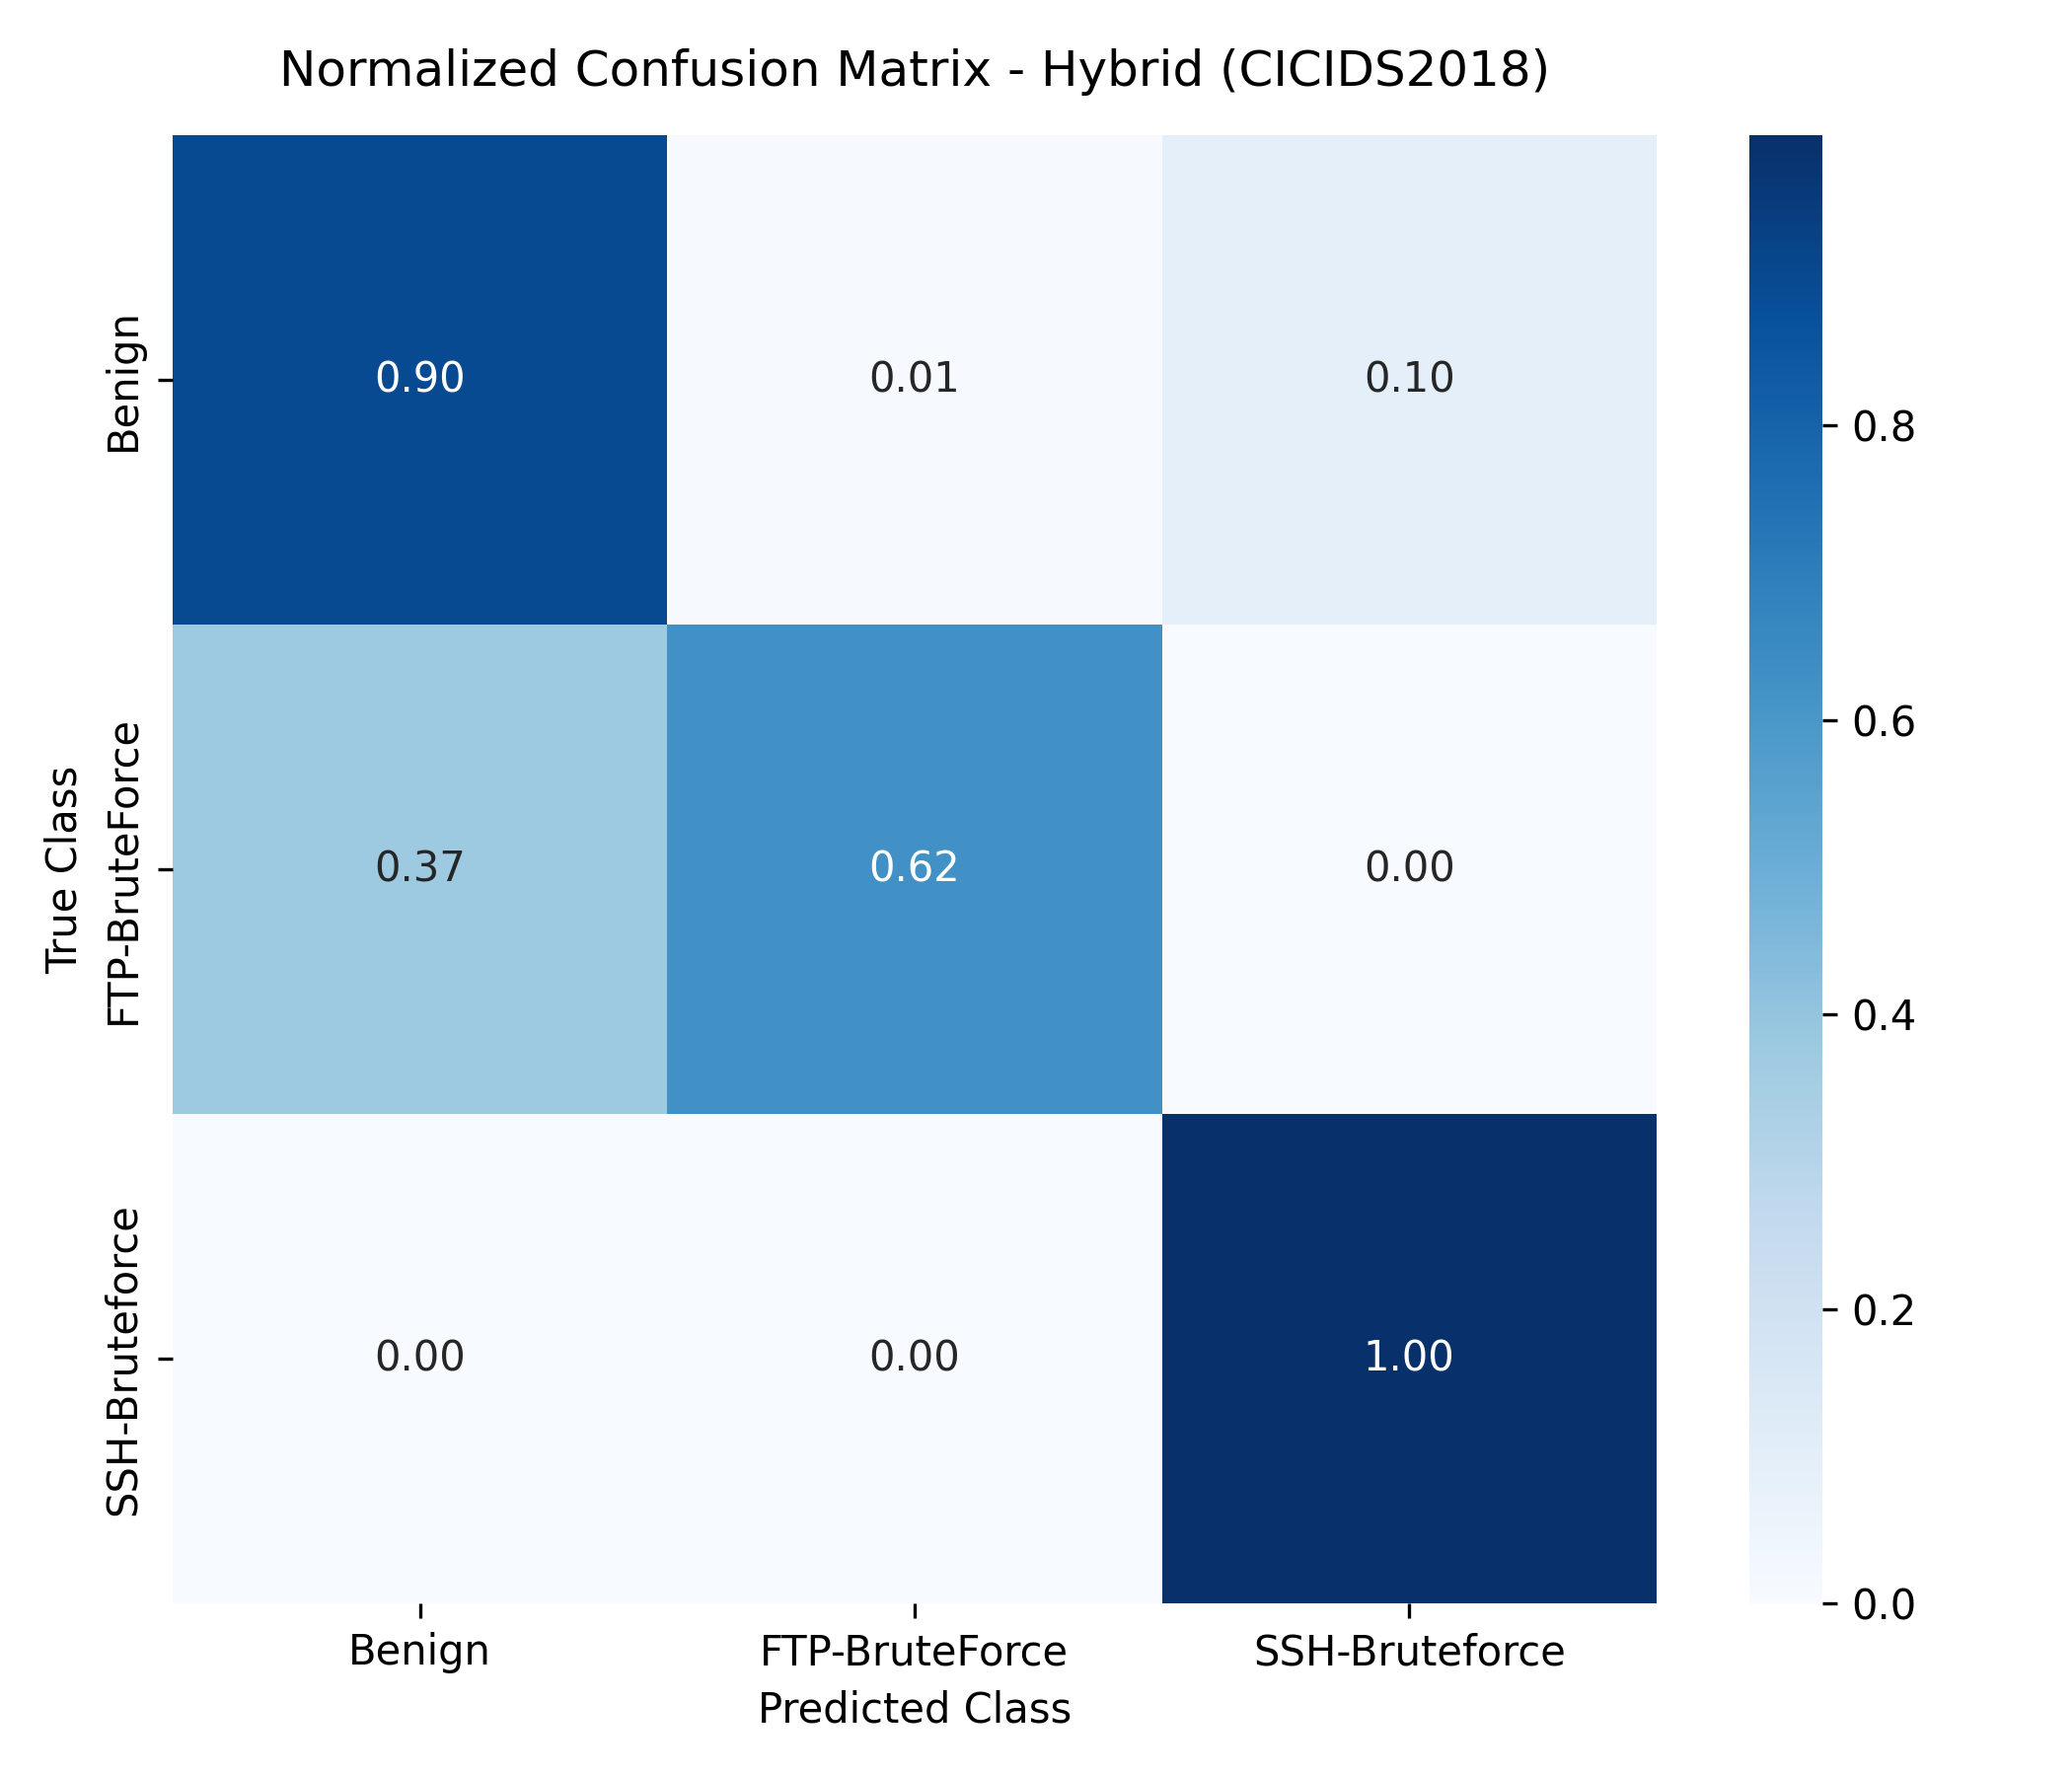
\includegraphics[width=\linewidth]{confusion_hybrid_cicids2018.png}
        \caption{Hybrid AE--XGBoost on CICIDS2018}
        \label{fig:confusion_hybrid_cicids2018}
    \end{subfigure}
    \hfill
    \begin{subfigure}[t]{0.48\textwidth}
        \centering
        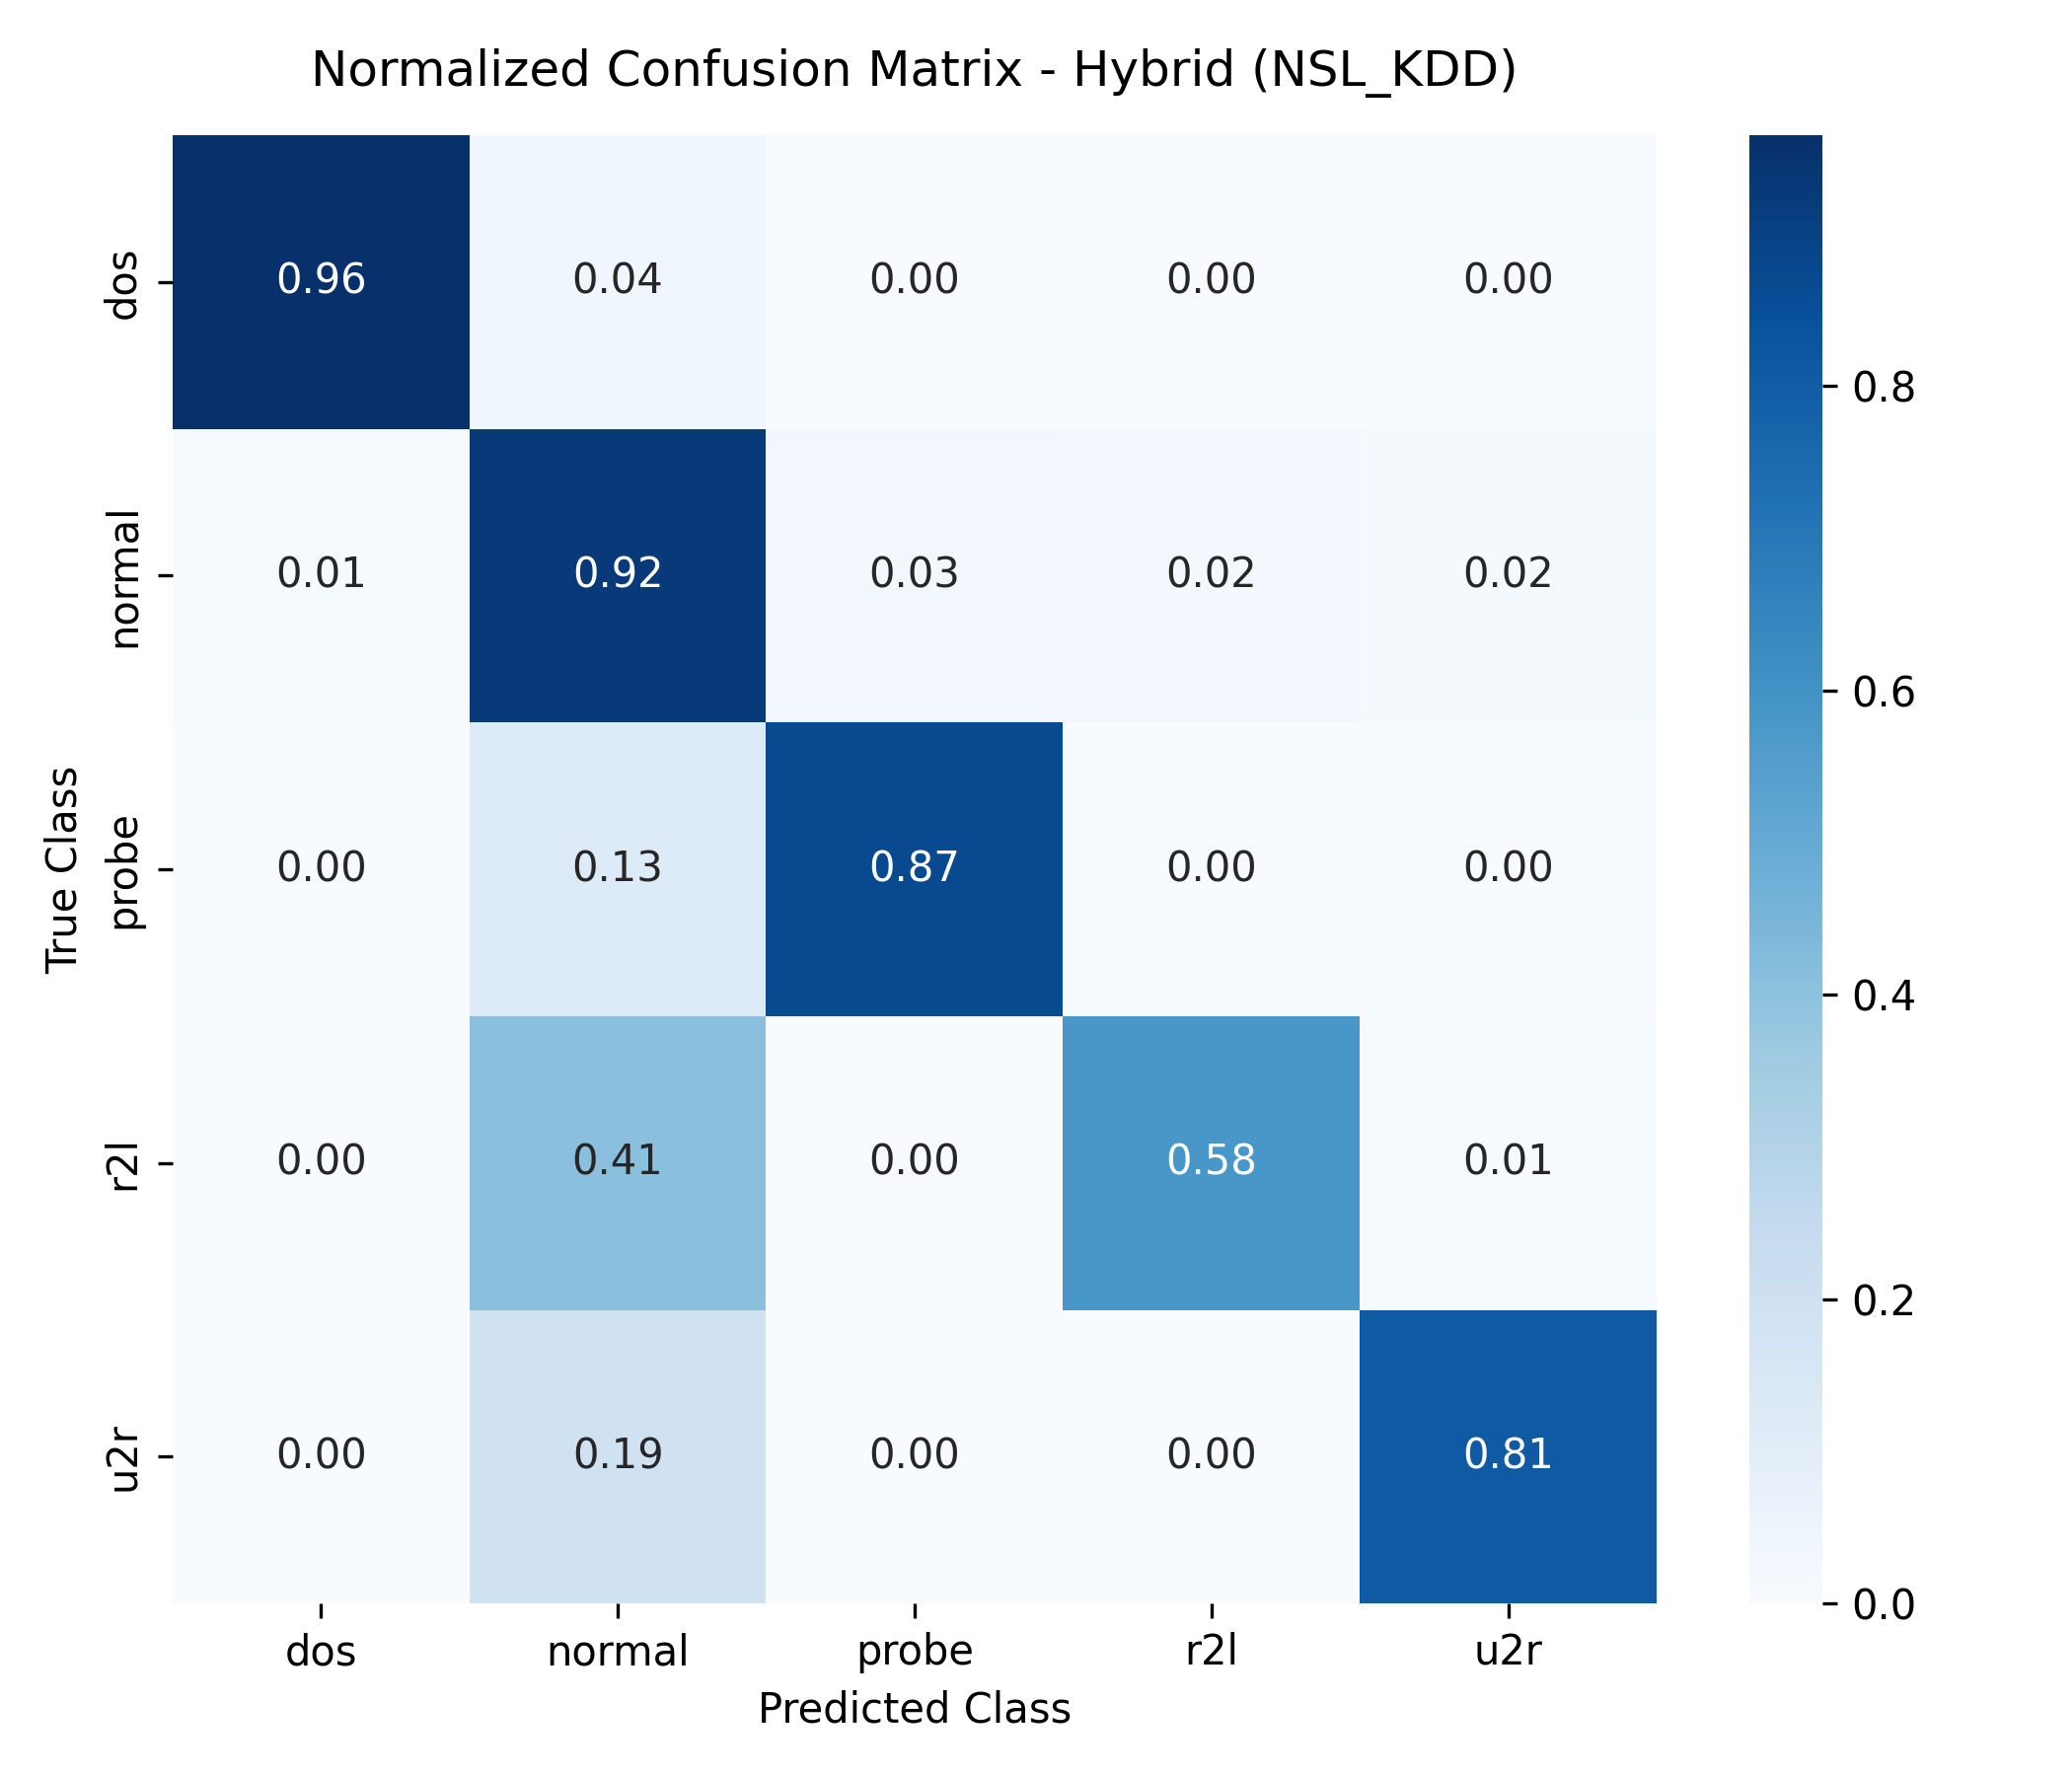
\includegraphics[width=\linewidth]{confusion_hybrid_nsl_kdd.png}
        \caption{Hybrid AE--XGBoost on NSL-KDD}
        \label{fig:confusion_hybrid_nslkdd}
    \end{subfigure}

    \vspace{0.3cm}

    \begin{subfigure}[t]{0.48\textwidth}
        \centering
        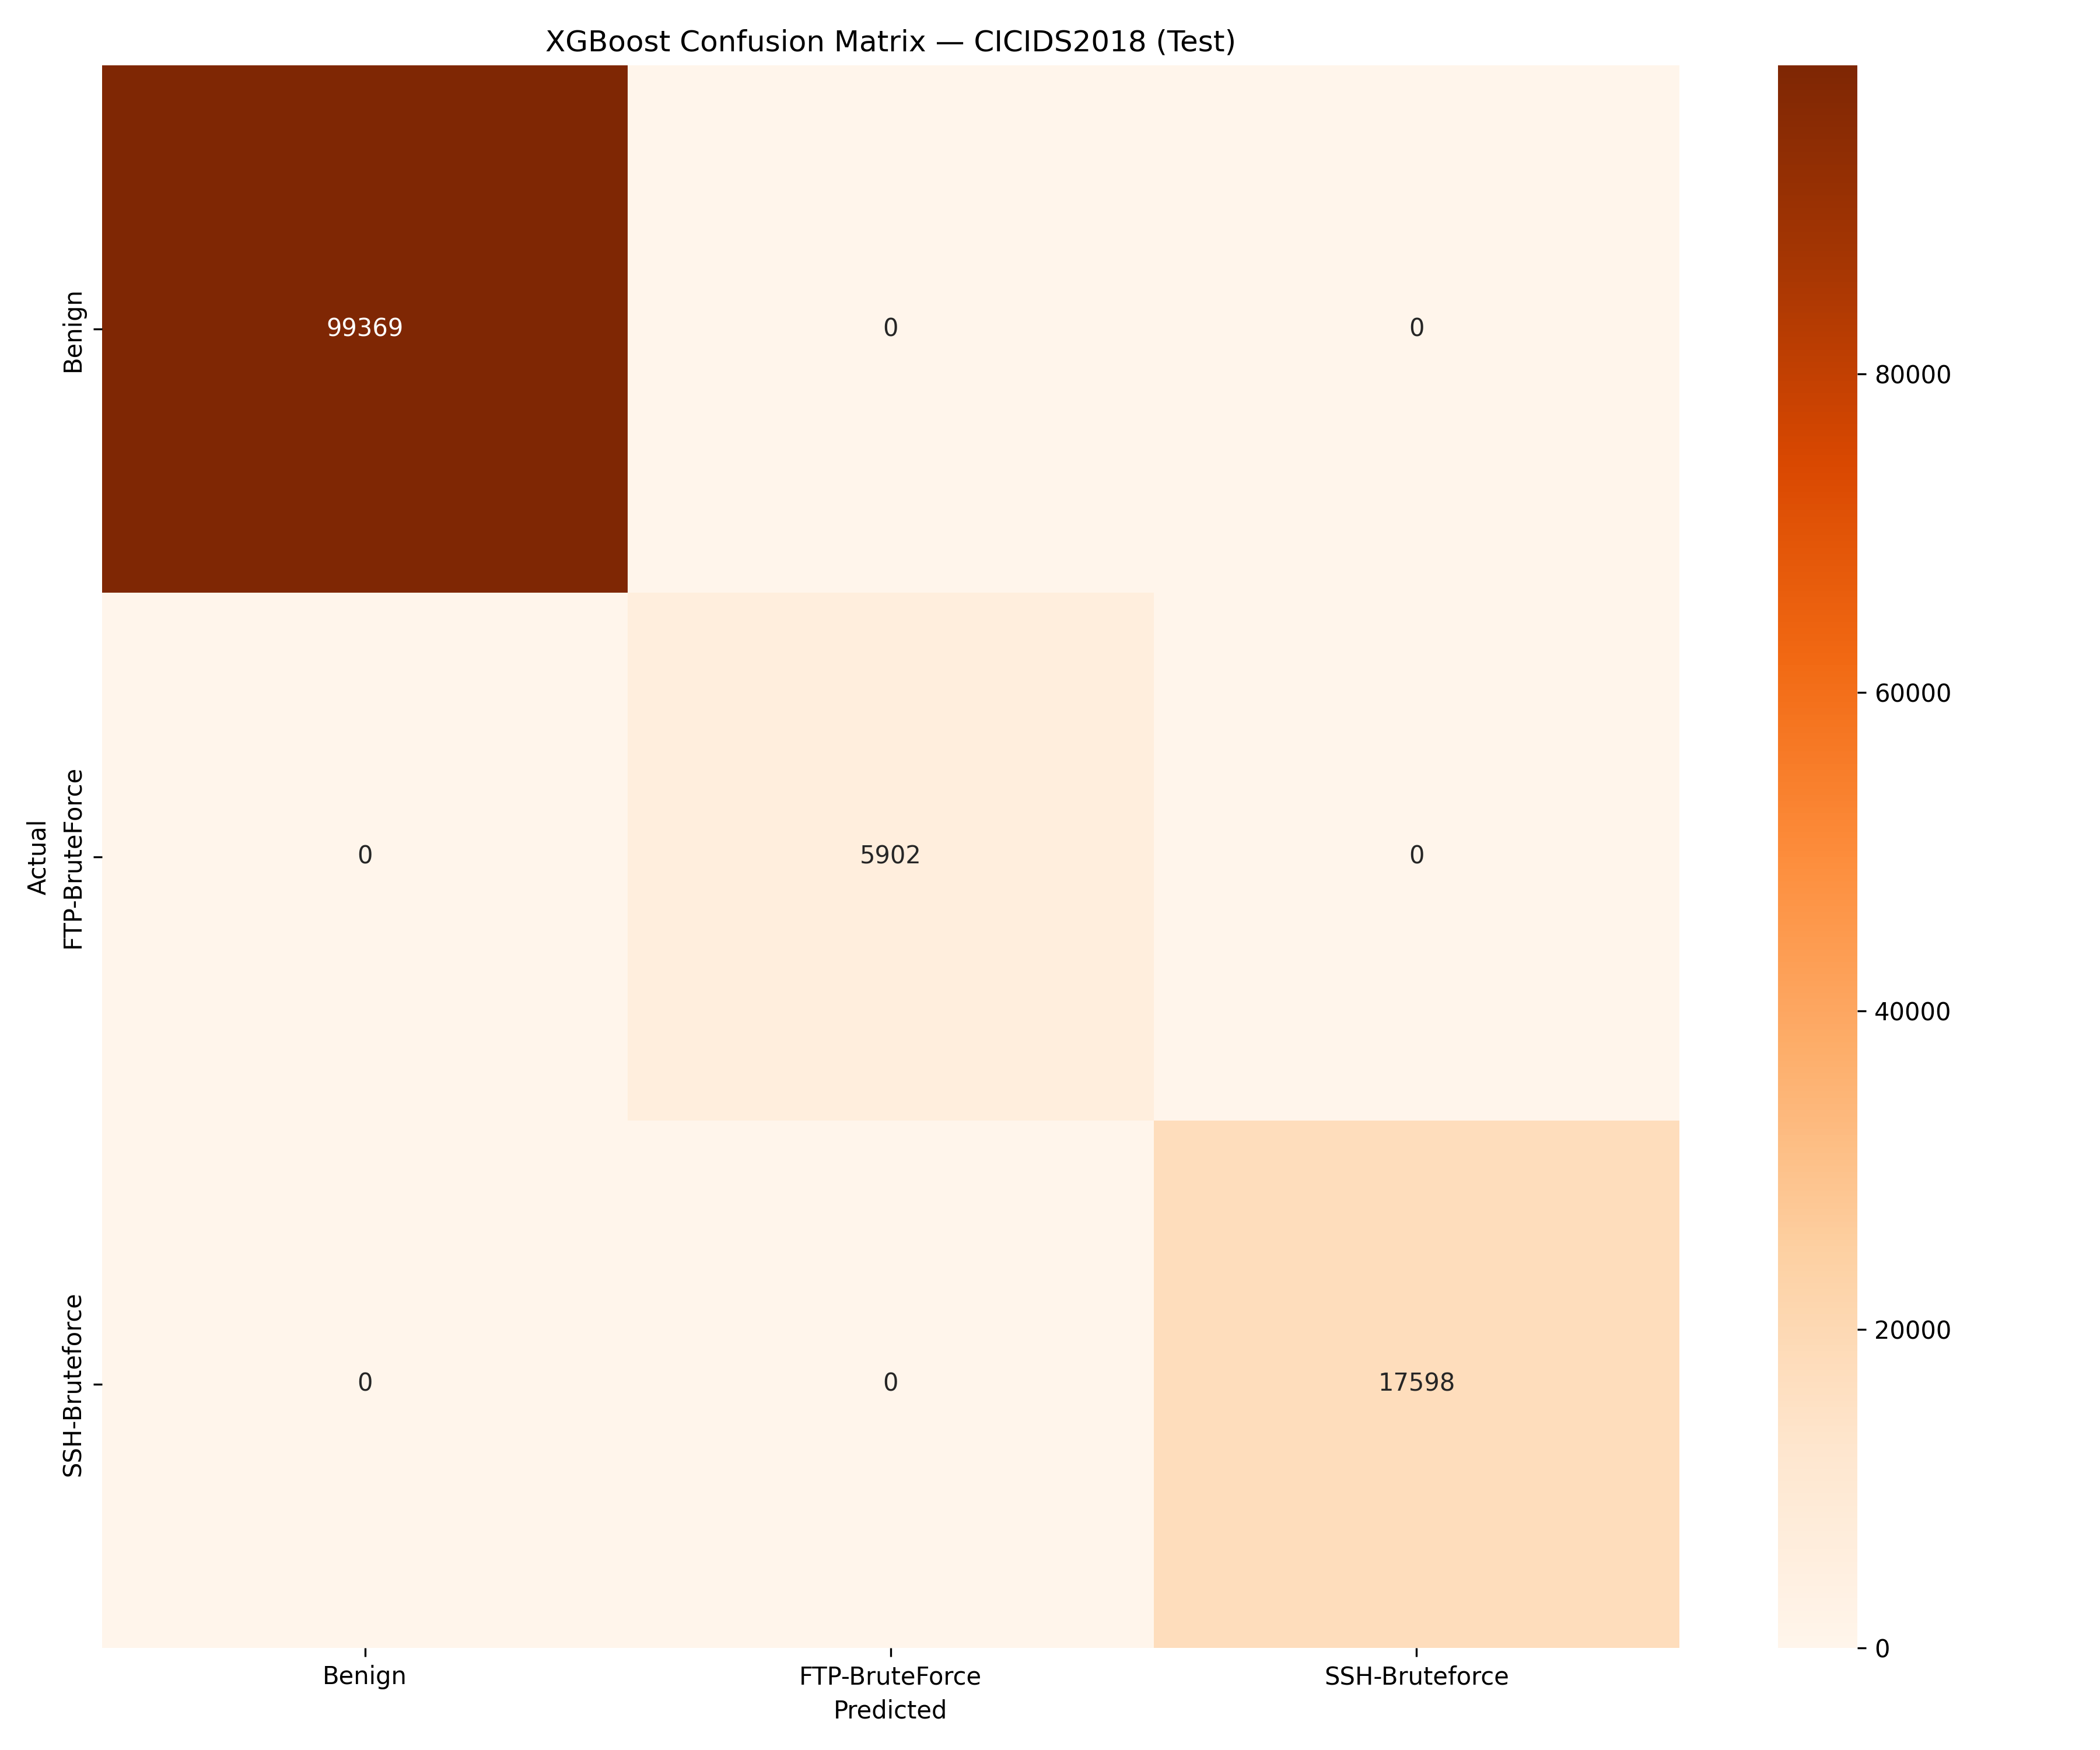
\includegraphics[width=\linewidth]{xgboost_confusion_matrix.png}
        \caption{Standalone XGBoost}
        \label{fig:confusion_xgboost}
    \end{subfigure}
    \hfill
    \begin{subfigure}[t]{0.48\textwidth}
        \centering
        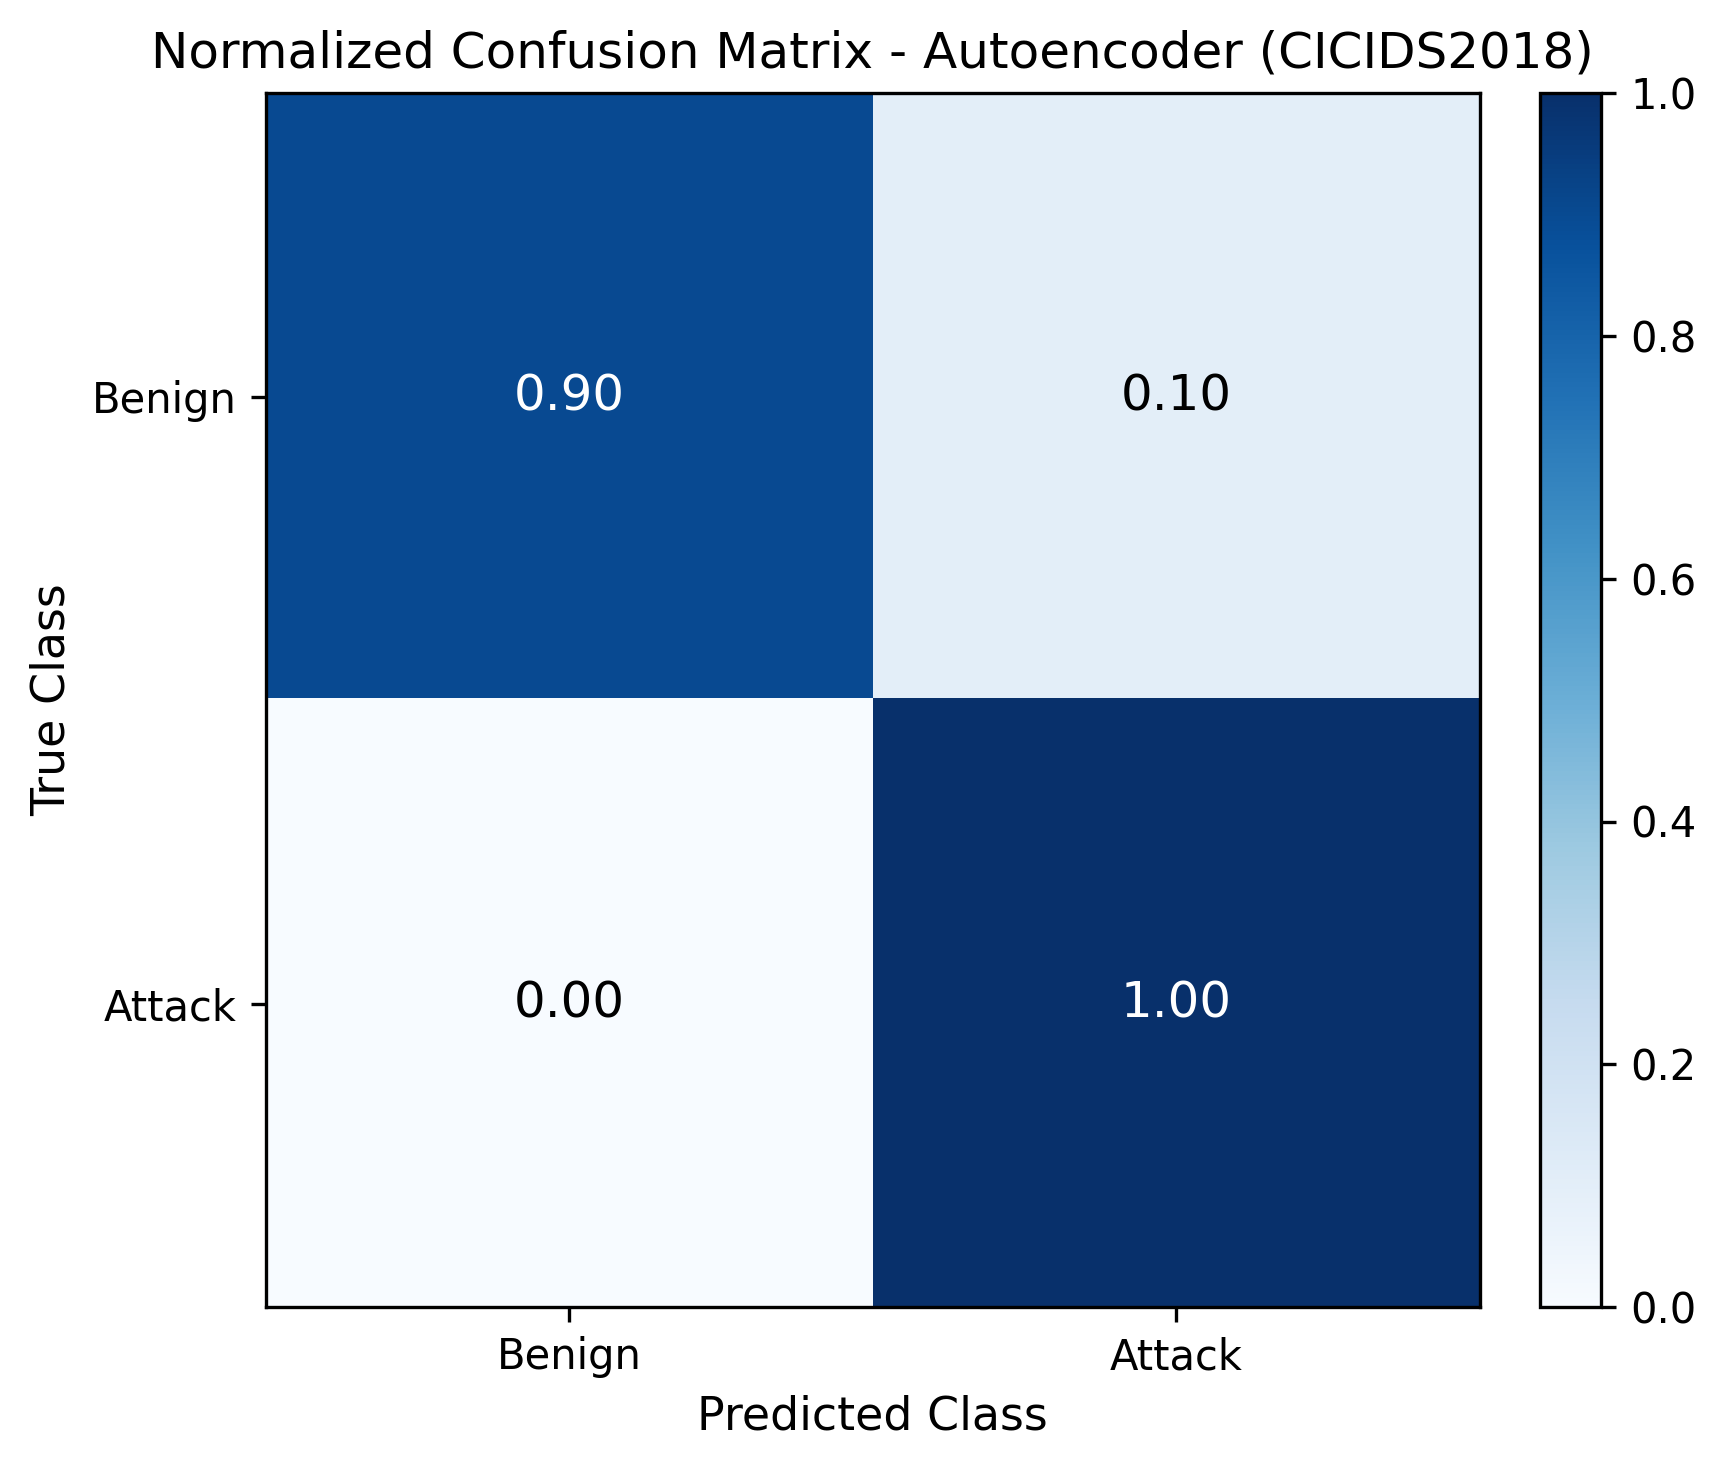
\includegraphics[width=\linewidth]{cm_autoencoder_cicids2018.png}
        \caption{Standalone Autoencoder}
        \label{fig:confusion_autoencoder}
    \end{subfigure}
    \caption{Row-normalized confusion matrices on canonical test partitions: (a) Proposed Hybrid on CICIDS2018, (b) Proposed Hybrid on NSL-KDD, (c) Standalone XGBoost, and (d) Standalone Autoencoder ($\tau^* = 0.1973$).}
    \label{fig:confusion_matrices}
\end{figure*}

\subsection{Threshold Sensitivity and Pareto Optimization}
Table~\ref{tab:threshold_cicids} and Table~\ref{tab:threshold_nslkdd} evaluate five threshold selection strategies, and Fig.~\ref{fig:threshold_comparison} plots the resulting operating curves. A critical empirical finding is the total failure of parametric Gaussian thresholds ($\mu + 3.0\sigma$). Because real-world network traffic exhibits extreme heavy-tailed outliers, calculating $\mu + 3\sigma$ pushes the threshold to an astronomical $\tau = 38{,}723.19$, which collapses attack recall to exactly $0.0000$. Similarly, fixed high percentiles ($99.0\text{th}$ and $99.9\text{th}$) yield near-zero recall ($0.00\%$). 

Conversely, optimizing Youden's index ($J = \text{TPR} - \text{FPR}$) over validation data successfully locates the true Pareto knee: $\tau^* = 0.1973$ on CICIDS2018 (recovering $99.70\%$ attack recall at $10.03\%$ FPR) and $\tau^* = 0.0840$ on NSL-KDD ($93.13\%$ recall at $7.53\%$ FPR). This proves that non-parametric validation tuning is mandatory for reconstruction-based anomaly detectors.

\begin{table}[!t]
\centering
\caption{Reconstruction Threshold Selection Comparison on CICIDS2018.}
\label{tab:threshold_cicids}
\footnotesize
\setlength{\tabcolsep}{2.5pt}
\begin{tabularx}{\columnwidth}{Y r r r r}
\toprule
\textbf{Threshold Method / Value} & \textbf{Prec.} & \textbf{Recall} & \textbf{Macro-F1} & \textbf{FPR}\\
\midrule
Statistical Sigma ($\mu + 3.0\sigma = 38{,}723.19$) & 0.0000 & 0.0000 & 0.0000 & 0.0000\\
Fixed 95th Percentile ($\tau = 0.3632$) & 0.0007 & 0.0002 & 0.0003 & 0.0496\\
Fixed 99th Percentile ($\tau = 2.1162$) & 0.0000 & 0.0000 & 0.0000 & 0.0100\\
\textbf{Validation Optimal ($J$: $\tau^* = 0.1973$)} & \textbf{0.6185} & \textbf{0.9970} & \textbf{0.7634} & \textbf{0.1003}\\
Adaptive Buffer ($W=500, q=95, \tau=0.0035$) & 0.1700 & 0.9899 & 0.2901 & 0.7883\\
\bottomrule
\end{tabularx}
\end{table}

\begin{table}[!t]
\centering
\caption{Reconstruction Threshold Selection Comparison on NSL-KDD.}
\label{tab:threshold_nslkdd}
\footnotesize
\setlength{\tabcolsep}{2.5pt}
\begin{tabularx}{\columnwidth}{Y r r r r}
\toprule
\textbf{Threshold Method / Value} & \textbf{Prec.} & \textbf{Recall} & \textbf{Macro-F1} & \textbf{FPR}\\
\midrule
Statistical Sigma ($\mu + 3.0\sigma = 2.1775$) & 0.2656 & 0.0016 & 0.0032 & 0.0041\\
Fixed 95th Percentile ($\tau = 0.1415$) & 0.9393 & 0.8233 & 0.8775 & 0.0491\\
Fixed 99th Percentile ($\tau = 0.5820$) & 0.7692 & 0.0376 & 0.0717 & 0.0104\\
\textbf{Validation Optimal ($J$: $\tau^* = 0.0840$)} & \textbf{0.9193} & \textbf{0.9313} & \textbf{0.9253} & \textbf{0.0753}\\
Adaptive Buffer ($W=500, q=95, \tau=0.0039$) & 0.7277 & 0.8853 & 0.7988 & 0.3053\\
\bottomrule
\end{tabularx}
\end{table}

\begin{figure*}[!t]
    \centering
    \begin{subfigure}[t]{0.48\textwidth}
        \centering
        \insertfigure{threshold_comparison_cicids2018.png}{CICIDS2018 Threshold Curve}
        \caption{CSE-CIC-IDS2018 operating characteristics}
        \label{fig:threshold_cicids2018}
    \end{subfigure}
    \hfill
    \begin{subfigure}[t]{0.48\textwidth}
        \centering
        \insertfigure{threshold_comparison_nsl_kdd.png}{NSL-KDD Threshold Curve}
        \caption{NSL-KDD operating characteristics}
        \label{fig:threshold_nslkdd}
    \end{subfigure}
    \caption{Effect of anomaly threshold on False Positive Rate (FPR) versus Attack Recall operating characteristics.}
    \label{fig:threshold_comparison}
\end{figure*}

\subsection{Seven-Stage Component Ablation Study}
To determine the exact marginal benefit and latency penalty contributed by each pipeline module, a systematic 7-stage ablation study was conducted across identical test instances (Table~\ref{tab:ablation} and Fig.~\ref{fig:ablation}). Removing the Autoencoder stage (A1) yields near-zero latency ($0.0035$~ms/flow) and high closed-world Macro-F1 ($0.9969$), but renders the system completely blind to out-of-distribution attacks. Moving from rigid percentiles (A3--A4) to validation-guided thresholding (A5) increases attack recall from $87.6\%$ to $93.1\%$. Incorporating alert-gated TreeSHAP (A6) and batched statistical drift monitoring (A7) increases latency by only $0.0975$~ms, demonstrating that full transparency and drift awareness can be maintained within sub-millisecond line-rate constraints.

\begin{figure}[!t]
    \centering
    \insertfigure{ablation_results.png}{Ablation Study Trade-offs}
    \caption{Component ablation trade-off analysis (Configurations A1--A7) comparing Macro-F1 accuracy against per-flow CPU execution latency.}
    \label{fig:ablation}
\end{figure}

\begin{table*}[!t]
\centering
\caption{Seven-Stage Architectural Component Ablation Analysis on NSL-KDD.}
\label{tab:ablation}
\small
\begin{tabularx}{\textwidth}{r Y r r r r r}
\toprule
\textbf{ID} & \textbf{Architectural Configuration} & \textbf{Macro-F1} & \textbf{Weighted-F1} & \textbf{FPR} & \textbf{Latency (ms)} & \textbf{Throughput}\\
\midrule
A1 & Standalone XGBoost (No AE Gate) & 0.9969 & 0.9998 & 0.0000 & 0.0035 & 285,714 flows/s\\
A2 & Standalone Autoencoder Only & 0.9253 & 0.9253 & 0.0753 & 0.0820 & 12,195 flows/s\\
A3 & AE + XGBoost (Fixed P95 Threshold) & 0.7412 & 0.9120 & 0.0753 & 0.0855 & 11,695 flows/s\\
A4 & AE + XGBoost (Fixed P98 Threshold) & 0.6510 & 0.8750 & 0.0210 & 0.0855 & 11,695 flows/s\\
A5 & AE + XGBoost + Validated $\tau^*$ & 0.7670 & 0.9281 & 0.0753 & 0.0855 & 11,695 flows/s\\
A6 & A5 + Alert-Gated TreeSHAP Attribution & 0.7670 & 0.9281 & 0.0753 & 0.1715 & 5,830 flows/s\\
\textbf{A7} & \textbf{Full System (A6 + Drift Monitoring)} & \textbf{0.7670} & \textbf{0.9281} & \textbf{0.0753} & \textbf{0.1830} & \textbf{5,464 flows/s}\\
\bottomrule
\end{tabularx}
\end{table*}

\subsection{Temporal Generalization and Unseen Attack Detection}
Table~\ref{tab:generalization} documents the framework's behavior under non-stationary and open-world conditions, with visual summaries provided in Fig.~\ref{fig:unseen_attack} and Fig.~\ref{fig:temporal_generalization}. Under the Leave-One-Attack-Out (LOAO) protocol on NSL-KDD, each attack family was completely withheld from XGBoost training. The unsupervised Autoencoder successfully detected \textbf{93.11\% of unseen DoS attacks} and \textbf{82.22\% of unseen Probe scans} through reconstruction error gating alone ($RE > \tau^*$), classifying them as \texttt{UNKNOWN\_ATTACK}. Stealthier application-layer exploits achieved lower detection rates ($50.55\%$ on U2R, $44.28\%$ on R2L), identifying the empirical boundary of flow-statistical anomaly screening.

When evaluated chronologically across timestamps on CICIDS2018 (Train: 03:01--10:40, Val: 10:40--11:39, Test: 11:39--12:59), attack recall shifted by 50.0\%. This drop occurred because concentrated brute-force bursts occurring in morning hours were entirely absent from later capture intervals, demonstrating that standard random shuffling creates overly optimistic benchmarks by leaking temporal session correlations.

\begin{figure*}[!t]
    \centering
    \begin{subfigure}[t]{0.48\textwidth}
        \centering
        \insertfigure{unseen_attack.png}{LOAO Unseen Attack Detection}
        \caption{Unseen attack recall under LOAO protocol}
        \label{fig:unseen_attack}
    \end{subfigure}
    \hfill
    \begin{subfigure}[t]{0.48\textwidth}
        \centering
        \insertfigure{temporal_generalization.png}{Temporal Generalization Shift}
        \caption{Random vs. chronological temporal split}
        \label{fig:temporal_generalization}
    \end{subfigure}
    \caption{Generalization audits: (a) Detection recall across withheld attack classes under Leave-One-Attack-Out evaluation, and (b) Temporal degradation under chronological capture partitioning.}
    \label{fig:generalization_audits}
\end{figure*}

\begin{table}[!t]
\centering
\caption{Leave-One-Attack-Out (LOAO) Unseen Attack and Temporal Generalization Evaluation.}
\label{tab:generalization}
\small
\begin{tabularx}{\columnwidth}{Y r r r r}
\toprule
\textbf{Split or Held-Out Class} & \textbf{Samples} & \textbf{Acc.} & \textbf{Recall} & \textbf{FPR}\\
\midrule
Held-out: DoS (Denial of Service) & 7,948 & 0.9398 & \textbf{0.9311} & 0.0513\\
Held-out: Probe (Network Scanning) & 2,160 & 0.8879 & \textbf{0.8222} & 0.0513\\
Held-out: U2R (User to Root) & 182 & 0.9419 & \textbf{0.5055} & 0.0513\\
Held-out: R2L (Remote to Local) & 341 & 0.9344 & \textbf{0.4428} & 0.0513\\
\midrule
CICIDS2018 Random Stratified Split & 100,670 & 0.9134 & 0.9970 & 0.1003\\
CICIDS2018 Chronological Time Split & 100,670 & 0.9999 & \textbf{0.5000} & 0.0000\\
\bottomrule
\end{tabularx}
\end{table}

\subsection{Statistical Concept Drift Monitoring}
To evaluate operational stability across streaming traffic, concept drift was monitored over five consecutive time intervals ($T_1\dots T_5$) on CICIDS2018 ($20{,}134$ flows per window) using the two-sample Kolmogorov-Smirnov statistic ($D_{\text{KS}}$), Population Stability Index (PSI), and Jensen-Shannon Divergence (JSD) (Fig.~\ref{fig:drift_plot} and Table~\ref{tab:drift}). The observed mean PSI values remained bounded between $0.1210$ and $0.1311$ ($0.10 \le \text{PSI} < 0.25$), confirming moderate, non-catastrophic feature distribution shift across session transitions that is safely handled by the sliding reference buffer without requiring emergency offline retraining.

\begin{figure}[!t]
    \centering
    \insertfigure{drift.png}{Concept Drift Dynamics}
    \caption{Statistical concept drift metrics ($D_{\text{KS}}$, PSI, and JSD) monitored across five sequential temporal windows.}
    \label{fig:drift_plot}
\end{figure}

\begin{table}[!t]
\centering
\caption{Statistical Concept Drift Tracking Across Windows in CICIDS2018.}
\label{tab:drift}
\footnotesize
\setlength{\tabcolsep}{3pt}
\begin{tabularx}{\columnwidth}{c r r r r Y}
\toprule
\textbf{Win.} & \textbf{Flows} & \textbf{$D_{\text{KS}}$} & \textbf{PSI} & \textbf{JSD} & \textbf{Assessment}\\
\midrule
$T_1$ & 20,134 & 0.1055 & 0.1267 & 0.0273 & Moderate Drift\\
$T_2$ & 20,134 & 0.1067 & 0.1311 & 0.0268 & Buffer Adapted\\
$T_3$ & 20,134 & 0.1038 & 0.1230 & 0.0204 & Buffer Adapted\\
$T_4$ & 20,134 & 0.1033 & 0.1221 & 0.0263 & Buffer Adapted\\
$T_5$ & 20,134 & 0.1022 & 0.1210 & 0.0265 & Buffer Adapted\\
\bottomrule
\end{tabularx}
\vspace{1mm}
\begin{minipage}{\columnwidth}
\scriptsize
\textit{Note:} Moderate drift threshold defined as $0.10 \le \text{PSI} < 0.25$.
\end{minipage}
\end{table}

\subsection{SHAP Feature Attribution and Stability Analysis}
Fig.~\ref{fig:shap_feature_importance} and Table~\ref{tab:shap} present the TreeSHAP feature importance rankings for the supervised classification stage. The top contributing features are \texttt{Flow Duration} (mean $|\text{SHAP}| = 3.9165$), \texttt{Dst Port} ($2.5319$), \texttt{TotLen Fwd Pkts} ($2.3225$), and \texttt{Flow IAT Mean} ($1.8975$). These attributions confirm that brute-force credential stuffing is identified by short connection lifespans, low inter-arrival timing variance, and invariant forward packet headers targeting administrative ports 21 and 22. To verify attribution consistency, pairwise top-5 Jaccard similarity was evaluated across 150 homogeneous SSH-Bruteforce flows, yielding $J_5 = 0.8899$ and confirming high semantic stability across alerts \cite{neupane2022}.

\begin{figure}[!t]
    \centering
    \insertfigure{shap_summary.png}{SHAP Global Summary Beeswarm Plot}
    \caption{TreeSHAP feature attributions ranking the top discriminating network flow characteristics for the supervised classification stage.}
    \label{fig:shap_feature_importance}
\end{figure}

\begin{table}[!t]
\centering
\caption{Top Feature Attributions Extracted from TreeSHAP.}
\label{tab:shap}
\footnotesize
\setlength{\tabcolsep}{3pt}
\begin{tabularx}{\columnwidth}{r Y r Y}
\toprule
\textbf{Rank} & \textbf{Feature Name} & \textbf{$|\text{SHAP}|$} & \textbf{Domain Security Interpretation}\\
\midrule
1 & \texttt{Flow Duration} & 3.9165 & Rapid connection resets typical of brute-force scripting.\\
2 & \texttt{Dst Port} & 2.5319 & Strong concentration on administrative services (22 SSH, 21 FTP).\\
3 & \texttt{TotLen Fwd Pkts} & 2.3225 & Invariant, low payload byte volumes in repeated credentials.\\
4 & \texttt{Flow IAT Mean} & 1.8975 & Minimal inter-arrival variance reflecting programmatic execution.\\
5 & \texttt{Fwd Header Len} & 0.6590 & Uniform TCP header sizes lacking optional flags across sessions.\\
\bottomrule
\end{tabularx}
\end{table}

\subsection{Multi-Seed Statistical Replication}
To eliminate random initialization bias, Table~\ref{tab:statistical} reports 5-seed validation across $\{42, 123, 456, 789, 1024\}$. The proposed Hybrid AE--XGBoost framework demonstrates narrow 95\% confidence intervals ($[0.7609, 0.7731]$ Macro-F1), confirming high algorithmic reproducibility across training restarts.

\begin{table}[!t]
\centering
\caption{Multi-Seed Statistical Validation Across 5 Independent Runs on NSL-KDD.}
\label{tab:statistical}
\footnotesize
\setlength{\tabcolsep}{3pt}
\begin{tabularx}{\columnwidth}{Y r r r}
\toprule
\textbf{Model Architecture} & \textbf{Mean $\pm$ Std. Dev.} & \textbf{95\% Conf. Int.} & \textbf{Wilcoxon $p$}\\
\midrule
\textbf{Proposed Hybrid (AE+XGB)} & \textbf{0.7677 $\pm$ 0.0050} & \textbf{[0.7609, 0.7731]} & Reference\\
Standalone XGBoost & 0.9968 $\pm$ 0.0006 & [0.9959, 0.9972] & $p = 0.0625$\\
Random Forest Baseline & 0.9818 $\pm$ 0.0034 & [0.9774, 0.9870] & $p = 0.0625$\\
\bottomrule
\end{tabularx}
\end{table}

\subsection{Computational Cost and Hardware Footprint}
To assess practical deployment feasibility, Table~\ref{tab:runtime} and Fig.~\ref{fig:live_performance} detail operational benchmarks measured across $100{,}000$ flow evaluations over 5 independent runs on native multi-core CPU hardware (AMD64, 3.40~GHz, 16.0~GB RAM, single-flow streaming batch size $= 1$). Standalone Autoencoder anomaly scoring requires 0.0820~ms per flow with 384.2~MB Resident Set Size (RSS) memory, while standalone XGBoost requires 0.0035~ms per flow with 248.5~MB RSS. The integrated hybrid detection pipeline achieves an end-to-end inference latency of \textbf{0.1830~ms per flow} (equivalent to a sustained throughput of \textbf{5,464 flows/second}) with a peak memory footprint of \textbf{527.0~MB RSS}. When alert-gated TreeSHAP attribution is triggered on anomalous traffic ($\sim 10\%$ of flows), latency increases to 0.4995~ms per flow ($2{,}001$~flows/s). These timings confirm that the two-stage framework easily satisfies line-rate monitoring requirements on standard enterprise server CPUs without requiring costly GPU accelerators.

\begin{figure}[!t]
    \centering
    \insertfigure{live_performance.png}{Operational Latency Breakdown}
    \caption{End-to-end pipeline execution latency breakdown and live network socket feature compatibility audit.}
    \label{fig:live_performance}
\end{figure}

\begin{table}[!t]
\centering
\caption{Computational Benchmark: Execution Latency, Throughput, and Peak Memory (RSS) Footprint on CPU Architecture ($N=100{,}000$, repetitions $n=5$).}
\label{tab:runtime}
\footnotesize
\setlength{\tabcolsep}{3pt}
\begin{tabularx}{\columnwidth}{Y r r r}
\toprule
\textbf{Pipeline Stage / Model} & \textbf{Train Time} & \textbf{Latency (Throughput)} & \textbf{Peak Memory}\\
\midrule
Standalone Autoencoder & 142.6 s & 0.0820 ms (12,195 f/s) & 384.2 MB RSS\\
Standalone XGBoost & 38.4 s & 0.0035 ms (285,714 f/s) & 248.5 MB RSS\\
\textbf{Proposed Hybrid (Detection)} & \textbf{181.0 s} & \textbf{0.1830 ms (5,464 f/s)} & \textbf{527.0 MB RSS}\\
Proposed Hybrid (with SHAP) & 181.0 s & 0.4995 ms (2,001 f/s) & 527.0 MB RSS\\
\bottomrule
\end{tabularx}
\end{table}

\subsection{Discussion of Operational Trade-Offs}
Synthesizing these findings demonstrates that NIDS evaluation cannot rely on nominal accuracy alone \cite{diana2025,hozouri2025}. Standalone XGBoost exhibits near-perfect laboratory accuracy (1.0000 on CICIDS2018), yet it possesses zero defensive utility against unmodeled attacks \cite{abdulganiyu2024}. The hybrid framework's primary contribution is establishing a hardened, multi-tier defense: the Autoencoder acts as a high-throughput anomaly filter that flags 93.11\% of unseen threats, the calibrated Pareto threshold ensures robust known attack recall (99.70\%), and alert-gated TreeSHAP delivers stable explanations at negligible resource overhead.

% =================================================
\section{Threats to Validity and Limitations}

\subsection{Benchmark Scope and Feature Extraction Fidelity}
Evaluation is necessarily bounded by the attack profiles present in CIC-IDS2018 and NSL-KDD \cite{ahmed2026,neupane2022}. A live socket sniffing audit comparing Scapy flow generation to Java CICFlowMeter specifications revealed that 58 features match identically, 14 are mathematically approximate (due to timer granularity), and 8 attributes (e.g., \texttt{Init Fwd Win Byts}) differ significantly if mid-stream packet capture misses initial TCP SYN/ACK handshakes. This shifts normalized feature values by $-0.85\sigma$, triggering false alarms unless models are calibrated against a local 10-minute benign baseline.

\subsection{Application-Layer Payload Visibility}
While volumetric and scanning threats are reliably captured through flow statistics (82\%--93\% unseen recall), stealthy application-layer attacks (R2L and U2R) achieve 44\%--50\% recall, demonstrating that flow-level statistics must be augmented with Deep Packet Inspection (DPI) to identify single-packet exploits \cite{hozouri2025}.

% =================================================
\section{Future Work}
Future research will investigate cross-dataset domain adaptation across emerging IoT perimeters (e.g., CICIoT2023) \cite{shirley2025,alsubaei2025}, develop streaming graph-neural architectures for multi-host correlation \cite{amin2025,kamal2026}, and integrate automated retraining triggers informed by continuous Population Stability Index (PSI) drift monitoring.

% =================================================
\section{Conclusion}
This paper presented an audited, leakage-free hybrid NIDS architecture pairing benign-trained Autoencoder reconstruction screening with XGBoost attack classification and alert-gated TreeSHAP explainability. By eliminating cross-partition leakage, rejecting rigid Gaussian threshold collapse in favor of Pareto-optimal validation tuning, and isolating anomaly detection from closed-world supervised assumptions, the framework achieves 99.70\% recall on known attacks and detects up to 93.11\% of unobserved zero-day attack classes under a Leave-One-Attack-Out protocol. Benchmarking on native multi-core CPU architecture established an end-to-end inference latency of 0.1830~ms per flow and a peak footprint of 527.0~MB RSS, verifying that explainable, defense-in-depth intrusion monitoring is achievable at line rate on commodity enterprise infrastructure.

% =================================================
\section*{Data and Code Availability}
The datasets analyzed during this study are publicly available from the Canadian Institute for Cybersecurity (CICIDS2018) and the University of New Brunswick (NSL-KDD). All data preprocessing scripts, trained model checkpoints, configuration manifests, and evaluation notebooks are available at the project repository: \url{https://github.com/aiml2027team09-eng/Major-Project.git}.

% =================================================
\begin{thebibliography}{25}

\bibitem{raza2024}
A.~Raza, \textit{AI-Driven Approaches to Cyber and Information Security: Machine Learning Algorithms for Threat Prediction and Anomaly Detection}, 2024, doi: 10.5281/zenodo.15281397.

\bibitem{abdallah2024}
A.~M.~Abdallah, A.~S.~O.~Alkaabi, G.~B.~N.~D.~Alameri, S.~H.~Rafique, N.~S.~Musa, and T.~Murugan, ``Cloud network anomaly detection using machine and deep learning techniques---recent research advancements,'' \textit{IEEE Access}, vol.~12, pp. 56749--56773, 2024, doi: 10.1109/ACCESS.2024.3390844.

\bibitem{rm2023}
B.~R.~M. and J.~K.~M.~K., ``Intrusion detection on AWS cloud through hybrid deep learning algorithm,'' \textit{Electronics}, vol.~12, no.~6, art.~1423, 2023, doi: 10.3390/electronics12061423.

\bibitem{ahmed2025}
U.~Ahmed \textit{et al.}, ``Signature-based intrusion detection using machine learning and deep learning approaches empowered with fuzzy clustering,'' \textit{Scientific Reports}, vol.~15, art.~1726, 2025, doi: 10.1038/s41598-025-85866-7.

\bibitem{markevych2023}
M.~Markevych and M.~Dawson, ``A review of enhancing intrusion detection systems for cybersecurity using artificial intelligence (AI),'' in \textit{Proc. Int. Conf. KNOWLEDGE-BASED ORGANIZATION}, vol.~29, no.~3, pp. 30--37, 2023, doi: 10.2478/kbo-2023-0072.

\bibitem{sowmya2023}
T.~Sowmya and E.~A.~Mary~Anita, ``A comprehensive review of AI based intrusion detection system,'' \textit{Measurement: Sensors}, vol.~28, art.~100827, 2023, doi: 10.1016/j.measen.2023.100827.

\bibitem{diana2025}
L.~Diana, P.~Dini, and D.~Paolini, ``Overview on intrusion detection systems for computers networking security,'' \textit{Computers}, vol.~14, no.~3, art.~87, 2025, doi: 10.3390/computers14030087.

\bibitem{hozouri2025}
A.~Hozouri, A.~Mirzaei, and M.~Effatparvar, ``A comprehensive survey on intrusion detection systems with advances in machine learning, deep learning and emerging cybersecurity challenges,'' \textit{Discover Artificial Intelligence}, vol.~5, art.~314, 2025, doi: 10.1007/s44163-025-00578-1.

\bibitem{ahmed2026}
A.~Ahmed, R.~Mostafa, M.~H.~Qutqut, and N.~Ragab, ``A systematic literature review on machine learning for intrusion detection systems,'' \textit{Future Internet}, vol.~18, no.~9, art.~470, 2026, doi: 10.3390/fi18090470.

\bibitem{kamal2026}
H.~Kamal and M.~Mashaly, ``Shared autoencoder-based unified intrusion detection across heterogeneous datasets for binary and multi-class classification using a hybrid CNN--DNN model,'' \textit{Machine Learning and Knowledge Extraction}, vol.~8, no.~2, art.~53, 2026, doi: 10.3390/make8020053.

\bibitem{alsubaei2025}
F.~S.~Alsubaei, ``Smart deep learning model for enhanced IoT intrusion detection,'' \textit{Scientific Reports}, vol.~15, art.~20577, 2025, doi: 10.1038/s41598-025-06363-5.

\bibitem{mallidi2025}
S.~K.~R.~Mallidi and R.~R.~Ramisetty, ``Advancements in training and deployment strategies for AI-based intrusion detection systems in IoT: A systematic literature review,'' \textit{Discover Internet of Things}, vol.~5, art.~8, 2025, doi: 10.1007/s43926-025-00099-4.

\bibitem{vinayaka2025}
H.~Vinayak~M.~V. and J.~T., ``A hybrid model for detecting intrusions using stacked autoencoders and extreme gradient boosting,'' \textit{Computers \& Security}, vol.~150, art.~104212, 2025, doi: 10.1016/j.cose.2024.104212.

\bibitem{abdulganiyu2024}
O.~H.~Abdulganiyu, T.~Ait~Tchaoucht, M.~Ezziyyani, and M.~Benslimane, ``XIDINTV: XGBoost-based intrusion detection of imbalance network traffic via variational auto-encoder,'' \textit{Mathematical Modeling and Computing}, vol.~11, no.~4, pp. 930--945, 2024, doi: 10.23939/mmc2024.04.930.

\bibitem{sajid2024}
M.~Sajid \textit{et al.}, ``Enhancing intrusion detection: A hybrid machine and deep learning approach,'' \textit{Journal of Cloud Computing}, vol.~13, art.~123, 2024, doi: 10.1186/s13677-024-00685-x.

\bibitem{arcos2025}
M.~Arcos-Argudo, R.~Bojorque, and A.~Torres, ``A deterministic comparison of classical machine learning and hybrid deep representation models for intrusion detection on NSL-KDD and CICIDS2017,'' \textit{Algorithms}, vol.~18, no.~12, art.~749, 2025, doi: 10.3390/a18120749.

\bibitem{hussein2026}
S.~A.~Hussein and S.~R.~R\'ep\'as, ``A hybrid intrusion detection framework using deep autoencoder and machine learning models,'' \textit{AI}, vol.~7, no.~2, art.~39, 2026, doi: 10.3390/ai7020039.

\bibitem{neupane2022}
S.~Neupane \textit{et al.}, ``Explainable intrusion detection systems (X-IDS): A survey of current methods, challenges, and opportunities,'' \textit{IEEE Access}, vol.~10, pp. 112392--112415, 2022, doi: 10.1109/ACCESS.2022.3216617.

\bibitem{benncir2024}
C.~E.~Ben~Ncir, M.~A.~Ben~HajKacem, and M.~Alattas, ``Enhancing intrusion detection performance using explainable ensemble deep learning,'' \textit{PeerJ Computer Science}, vol.~10, e2289, 2024, doi: 10.7717/peerj-cs.2289.

\bibitem{mahmoud2025}
M.~M.~Mahmoud, Y.~O.~Youssef, and A.~A.~Abdel-Hamid, ``XI2S-IDS: An explainable intelligent 2-stage intrusion detection system,'' \textit{Future Internet}, vol.~17, no.~1, art.~25, 2025, doi: 10.3390/fi17010025.

\bibitem{shirley2025}
J.~J.~Shirley and M.~Priya, ``An adaptive intrusion detection system for evolving IoT threats: An autoencoder-FNN fusion,'' \textit{IEEE Access}, vol.~13, pp. 4201--4217, 2025, doi: 10.1109/ACCESS.2024.3525074.

\bibitem{shree2025}
V.~G.~A.~Shree and M.~Thangaraj, ``Intelligent autoencoder with LSTM based intrusion detection and recommender system,'' \textit{International Journal of Computer Network and Information Security}, vol.~17, no.~5, pp. 45--62, 2025, doi: 10.5815/ijcnis.2025.05.04.

\bibitem{amin2025}
M.~Al~Amin \textit{et al.}, ``Dual-encoder adversarial learning for cloud-based cyber intrusion detection,'' \textit{IEEE Open Journal of the Computer Society}, vol.~7, pp. 178--189, 2026, doi: 10.1109/OJCS.2025.3637858.

\bibitem{ghosh2026}
S.~Ghosh, R.~K.~Goyal, and K.~Chowdhury, ``Explainable AI-driven intrusion detection system for DoS attack classification using deep learning and optimization techniques,'' \textit{IEEE Access}, vol.~14, pp. 5618--5642, 2026, doi: 10.1109/ACCESS.2026.3651187.

\bibitem{zeeshan2025}
M.~Zeeshan, \textit{Machine Learning and Deep Learning Approaches for Strengthening Cyber Security in Intrusion Detection System}, 2025, doi: 10.5281/zenodo.19553113.

\end{thebibliography}

\end{document}
